\documentclass[12pt]{report}

\usepackage{graphicx, color}
\usepackage[T1]{fontenc}
\usepackage[utf8]{inputenc}
\usepackage[english]{babel}
\usepackage[a4paper,margin=2cm]{geometry}
\usepackage{amsmath}
\usepackage{amssymb}
\usepackage{url}

% hyperref must be loaded (almost) last so it can patch the other packages.
\usepackage[colorlinks=true,
            linkcolor=blue,    % internal links (sections, figures, equations)
            citecolor=blue,    % \cite links
            urlcolor=blue,     % \url / \href links
            linktoc=all]{hyperref}
\usepackage{cleveref} % optional: \cref/\Cref smart references; load AFTER hyperref


\newcommand{\red}[1]{{\color{red}{#1}}}



\begin{document}





\begin{titlepage}



\newcommand{\HRule}{\rule{\linewidth}{0.5mm}} % Defines a new command for the horizontal lines, change thickness here

\center % Center everything on the page

 

%----------------------------------------------------------------------------------------

%	HEADING SECTIONS

%----------------------------------------------------------------------------------------


\textsc{\Large MSc Artificial Intelligence}\\[0.2cm]

\textsc{\Large Master Thesis}\\[0.5cm] 



%----------------------------------------------------------------------------------------

%	TITLE SECTION

%----------------------------------------------------------------------------------------



\HRule \\[0.4cm]

{ \huge \bfseries Geometrically-Aware Hyperbolic Residual-Quantized Variational AutoEncoders}\\[0.4cm] % Title of your document

\HRule \\[0.5cm]

 

%----------------------------------------------------------------------------------------

%	AUTHOR SECTION

%----------------------------------------------------------------------------------------



by\\[0.2cm]

\textsc{\Large Alessio Colombo}\\[0.2cm] %you name

15387569\\[1cm]





%----------------------------------------------------------------------------------------

%	DATE SECTION

%----------------------------------------------------------------------------------------



{\Large \today}\\[1cm] % Date, change the \today to a set date if you want to be precise



36 ETCs\\ %

January 6th 2026 to June 19th 2026 \\[1cm]%



%----------------------------------------------------------------------------------------

%	COMMITTEE SECTION

%----------------------------------------------------------------------------------------

\begin{minipage}[t]{0.4\textwidth}

\begin{flushleft} \large

\emph{Supervisor:} \\

Melika Ayoughi% Supervisor's Name

\end{flushleft}

\end{minipage}

~

\begin{minipage}[t]{0.4\textwidth}

\begin{flushright} \large

\emph{Examiner:} \\

\red{Dr A  \textsc{Person}}\\

\vspace{0.5cm}

\emph{Second reader:} \\

\red{Dr A  \textsc{Person}}\\

\end{flushright}

\end{minipage}\\[2cm]



%----------------------------------------------------------------------------------------

%	LOGO SECTION

%----------------------------------------------------------------------------------------





\includegraphics[width=10cm]{uvalogo_regular_p_nl.eps}

 

%----------------------------------------------------------------------------------------



\vfill % Fill the rest of the page with whitespace

\end{titlepage}

\pagenumbering{roman}

\tableofcontents

\begin{abstract}
\red{Provide a short overview and description of your thesis here.}
\end{abstract}

\pagenumbering{arabic}

\chapter{Introduction}
\label{chap:intro}

Much of the recent progress in generative modelling rests on a single design pattern: rather than model a continuous signal directly, one first compresses it into a short sequence of \emph{discrete} tokens and then trains a powerful sequence model --- an autoregressive transformer or a discrete diffusion model --- over those tokens. This tokenize-then-generate recipe now underpins state-of-the-art systems for images, audio, video, and even sequential recommendation, because it converts heterogeneous, high-dimensional data into the uniform symbolic interface that large sequence models consume most effectively. The component that produces those tokens is therefore decisive: the quality, capacity, and structure of the discrete code determine what the downstream model can ever learn. The dominant way to learn such codes is Vector Quantization (VQ) \cite{originalvq}, revived for deep learning by the VQ-VAE \cite{vqvae}, which inserts a learnable codebook as a discrete bottleneck in an autoencoder and trains it end-to-end through the Straight-Through Estimator (STE) \cite{straight_through_estimator}.

A single codebook, however, scales poorly: reaching high fidelity demands an exponentially large dictionary or a longer token grid, the first hard to optimize and the second quadratically expensive for the downstream transformer \cite{soundstream}. \emph{Residual Vector Quantization} (RVQ) resolves this by quantizing in $D$ successive stages, each coding the residual error left by the previous one \cite{soundstream, lee2022rqvae}. The aggregate code is the sum of the per-stage codewords, which manufactures a virtual dictionary of size $K^D$ at the cost of $D$ small ones, and --- more importantly for what follows --- imposes a \emph{coarse-to-fine} structure: early stages capture global content and later stages add progressively finer detail, so truncating the code tuple yields a graceful, semantically coherent approximation. This coarse-to-fine cascade is the backbone of modern neural audio codecs such as SoundStream \cite{soundstream} and EnCodec \cite{encodec}, of high-resolution image tokenizers \cite{lee2022rqvae}, and of the semantic-ID paradigm in generative recommendation \cite{tiger}.

The defining property of RVQ is thus that it does not merely discretize data: it imposes a \emph{hierarchy} on it. Each input is represented by an ordered tuple of codes whose prefixes form a tree of ever-coarser approximations. Yet every stage of this construction is carried out in Euclidean space, and Euclidean geometry is flat: the volume of a ball grows only polynomially with its radius, leaving no room to place an exponentially branching set of descendants equidistant from a common ancestor without crowding or distortion. Hyperbolic geometry is the natural remedy. In a space of constant negative curvature, ball volume grows \emph{exponentially} with radius, matching the growth of a tree's node count, and any weighted tree embeds into the Poincar\'e ball with arbitrarily low distortion in as few as two dimensions, whereas a faithful Euclidean embedding needs a dimension that grows with the tree \cite{cannon1997hyperbolic, sala2018representation, nickel2017poincare}. Placing the codebooks of a residual quantizer on a hyperbolic manifold therefore supplies an inductive bias precisely aligned with the coarse-to-fine hierarchy that RVQ already induces.

A line of recent work has begun to act on this intuition, lifting single-stage VQ \cite{hypervq, hvqvae} and, closest to us, the residual cascade itself \cite{hrqvae, hyprqvae_recsys} onto the Poincar\'e ball. Our central observation is that these methods are \emph{hyperbolic in name more than in operation}: they exploit the geometry only where it is cheap --- placing points inside the ball and measuring nearest-neighbour assignments by geodesic distance --- while the operations that actually carry the learning signal remain Euclidean. They put the representation on the manifold but train it off it. Concretely, they place the representations on the manifold yet leave the \emph{machinery that trains them} essentially Euclidean. The non-differentiable quantizer still propagates its gradient through the identity-Jacobian STE, which copies a gradient from the chosen codeword to the encoder as though the two lay in the same flat tangent space; codebooks are still updated with k-means and exponential-moving-average rules that ignore the Fr\'echet-mean structure of the curved space; and the residual recursion is obtained by a direct transliteration of Euclidean subtraction and summation into their M\"obius counterparts. Two operations sit at the very heart of residual quantization, and both are left geometrically incorrect by this transplant: \emph{(i)} the gradient that the quantizer must deliver back to the encoder, and \emph{(ii)} the residual recursion that decomposes the signal coarse-to-fine. Compounding the issue, these approaches were validated almost exclusively in the \emph{shallow} regime ($n_q\!\approx\!4$), exactly where both defects are mildest and a deep cascade's pathologies never surface.

This thesis closes that gap by treating residual quantization as a first-class operation on the manifold rather than a Euclidean procedure performed on hyperbolic coordinates. Our analysis turns on a structural fact that, to our knowledge, has not been articulated before. Euclidean RVQ is depth-stable for a precise reason: the additive update $r_i = r_{i-1}-q_i$ composed with the identity STE produces an exact Jacobian cancellation, $\partial r_i/\partial r_{i-1}=I-I=0$, that we call the \emph{Euclidean firewall}. The firewall is what guarantees that, however deep the stack, the encoder receives exactly one clean copy of the reconstruction gradient and only the coarsest commitment term, leaving the model's training signal independent of depth. On the Poincar\'e ball this cancellation breaks: the M\"obius update carries mismatched conformal factors, the firewall \emph{leaks}, and reconstruction \emph{and} commitment gradients accumulate across stages, each filtered through a different-length product of leak matrices whose norm grows toward the boundary. The naive per-stage repair --- making each transport geometrically exact --- only makes matters worse, because it injects the diverging conformal factors of the metric into every stage and the encoder gradient explodes with depth. Per-stage geometric correctness and depth stability are thus in direct tension, and resolving it requires abandoning the per-stage view entirely. In parallel, the residual recursion suffers a distinct, purely \emph{forward} failure: because M\"obius addition is neither commutative nor associative, the transliterated subtract-then-resum convention used by prior work does not telescope, so the tracked residual silently drifts away from the true reconstruction error and the deeper codebooks are fitted to a target that no longer represents what they are meant to encode.

Out of this analysis we build a single, geometry-first residual-quantization module that is agnostic to modality, architecture, and stack depth, which we name \textbf{GHRQ} (Geometry-aware Hyperbolic Residual Quantization).\footnote{In the experimental chapters the fully-featured instantiation of GHRQ is referred to by its configuration label \emph{A4}; the two names denote the same method.} GHRQ rests on three pillars. First, \emph{Hyperbolic Residual Aggregation} (HRA) replaces the transliterated cascade with the unique pairing of left M\"obius subtraction and reverse-nested aggregation that the gyrogroup cancellation law makes an exact inverse pair, so the residuals telescope and the codes recompose to the encoder point on the ball. Second, the \emph{block-level discounted hyperbolic straight-through estimator} (d-HSTE) removes the geometric correction from the recursion and instead transports a \emph{single} aggregate reconstruction gradient from the block output to the encoder in one parallel-transport hop, with the per-stage codes detached to seal the leak and a Riemannian discount that keeps the lone transport finite near the boundary; this reproduces, on the curved manifold, exactly the depth-independent single-copy routing that the Euclidean firewall grants for free. Third, a set of \emph{numerical-stabilization} techniques --- a cancellation-free reformulation of the gyration in the backward pass, together with explicit boundary controls --- keeps the estimator well-conditioned in the high-curvature regime where the geometry is most expressive but the conformal factors diverge. The module is a drop-in replacement for a Euclidean residual quantizer, selected entirely through flags and reducing exactly to standard RVQ at curvature $c=0$.

\paragraph{Contributions.} In summary, this thesis makes the following contributions:
\begin{itemize}
    \item \textbf{The Euclidean firewall and its leak.} We identify the exact Jacobian cancellation that makes Euclidean RVQ depth-stable, show that it leaks on the Poincar\'e ball so that both reconstruction and commitment gradients accumulate with depth, and prove that the obvious per-stage geometric correction trades this leak for a depth-driven gradient explosion --- establishing that per-stage correctness and depth stability cannot be reconciled inside the recursion (Chapter~\ref{chap:methods}).
    \item \textbf{The block-level d-HSTE.} We derive a hyperbolic straight-through estimator that routes one geometrically correct, depth-independent gradient from the aggregate reconstruction to the encoder, combining single-hop parallel transport, code detachment, and a Riemannian discount, and show it is the curved analogue of the Euclidean firewall's routing (\S\ref{sec:hste}).
    \item \textbf{Hyperbolic Residual Aggregation (HRA).} We show that the M\"obius transliteration adopted by prior hyperbolic residual quantizers fails to telescope, and identify the unique left-subtraction / reverse-nested aggregation pairing that restores an exact coarse-to-fine decomposition on the ball (\S\ref{sec:residagg}).
    \item \textbf{Numerical stabilization.} We give a cancellation-free reformulation of the backward-pass gyration and the boundary controls required to train deep hyperbolic stacks without collapse (\S\ref{sec:blockste}, Appendix~\ref{app:gyration}).
    \item \textbf{A broad empirical study.} We evaluate the same module across four modalities --- image reconstruction and generation, language-hierarchy embedding, sequential recommendation, and neural audio coding --- spanning the shallow ($n_q\!=\!4$) regime of prior work and the deep ($n_q\!=\!12$) regime where the firewall leak becomes decisive. To our knowledge this includes the first hyperbolic residual-quantized \emph{neural audio codec} (Chapters~\ref{chap:expsetup}--\ref{chap:experiments}).
\end{itemize}

\paragraph{Scope of the findings.} We report these results without overstating them. Where the data carries a latent hierarchy, hyperbolic curvature consistently helps: it recovers the CIFAR-100 superclass taxonomy from unsupervised codes, owns the trainable sweet spot on WordNet hypernymy, and improves downstream recommendation. The block-level estimator earns its keep precisely where predicted, keeping the deep $n_q\!=\!12$ audio codec trainable where the naive lift degrades, and the HRA cascade telescopes to a near-zero on-ball reconstruction residual across every domain. The one claim the evidence does \emph{not} support is hyperbolic-as-a-better-compressor: a Euclidean residual quantizer wins raw reconstruction on every image dataset and at audio scale, and on a task with no hierarchy to exploit GHRQ's contribution reduces to collapse-avoidance. The defensible thesis is therefore not that curvature compresses better, but that a \emph{correctly} hyperbolic residual quantizer is robust and depth-trainable, and that it reorganizes the code space toward hierarchy and toward better downstream and generative tokens --- trading a modest amount of distortion for structure on exactly the data where structure exists.

\paragraph{Thesis outline.} Chapter~\ref{chap:background} reviews the discrete-representation and hyperbolic-geometry background on which the method builds. Chapter~\ref{chap:methods} develops GHRQ: the firewall analysis (\S\ref{sec:firewall}) and the block-level d-HSTE (\S\ref{sec:hste}), the HRA aggregation (\S\ref{sec:residagg}), and the hyperbolic training objectives. Chapter~\ref{chap:expsetup} specifies the four tasks, datasets, architectures, and the three quantizer configurations compared throughout; Chapter~\ref{chap:experiments} reports and interprets the results. We close with a discussion of limitations and directions for combining the leaked residual signal with the block-level estimator.

\chapter{Related Work}

This chapter reviews the literature relevant to our work, placing our contributions in a broader context by first discussing discrete representation learning through vector quantization (\S\ref{sec:vq}), then examining its hierarchical version through residual quantization (\S\ref{sec:rvq}), and finally reviewing its recent extension to hyperbolic geometry.(\S\ref{sec:hyperbolic_repr}).

\section{Vector Quantization}
\label{sec:vq}
add why deep learning is good for quantization and vice versa. more specific title.
Vector quantization (VQ) has a long history in signal processing as a method for lossy data compression \cite{originalvq}. The modern revival of VQ in deep learning was catalyzed by the VQ-VAE \cite{vqvae}, which introduced a discrete bottleneck into the variational autoencoder framework. By mapping continuous encoder outputs to the nearest vector in a learnable codebook, VQ-VAE enabled the learning of compact discrete representations suitable for downstream generative modeling. Since the nearest-neighbor assignment is non-differentiable, gradient flow through the quantization step is enabled by the Straight-Through Estimator (STE) \cite{straight_through_estimator}, which copies gradients from the decoder input directly to the encoder output, effectively treating the quantization as the identity function during backpropagation.

A practical obstacle in training such models is codebook collapse \cite{collapse_1, collapse_2}, where only a small fraction of codewords are ever selected while the rest receive no gradient signal and remain unused, sharply limiting the effective capacity of the discrete bottleneck. To mitigate this well-known issue, various remedies have been proposed, ranging from heuristic codebook resets and exponential moving average (EMA) updates to principled variational relaxations (e.g., HQ-VAE \cite{hqvae}) and alternative discrete bottlenecks like Gumbel-Softmax \cite{gumbelvq} and Finite Scalar Quantization \cite{finitescalarquantizationfsq}.

While single-stage VQ enables high-fidelity synthesis and generation, achieving high representational capacity requires exponentially large codebooks, which are difficult to optimize \cite{soundstream}. Alternatively, increasing the spatial sequence length of discrete tokens creates a computational bottleneck for downstream autoregressive transformers, which scale quadratically with sequence length. These limitations motivate the multi-stage residual approach discussed next.

\section{Residual Vector Quantization}
\label{sec:rvq}

Residual Vector Quantization (RVQ) extends the single-stage VQ paradigm by quantizing the representation in multiple successive stages \cite{soundstream}. At each stage $d$, the residual error from the previous stage is quantized using a dedicated codebook, and the new residual is computed by subtracting the selected codeword. The final representation is the sum of all selected codewords across the $D$ stages. This decomposition effectively constructs a virtual codebook with exponential representational capacity ($K^D$ for $D$ codebooks of size $K$) without expanding the physical memory footprint or the spatial sequence length of the discrete tokens. A single input data is thus represented not by a single discrete token, but by an ordered tuple of $D$ indices, where early entries capture global, macro-level information and later entries encode progressively finer details \cite{lee2022rqvae}.

RQ-VAE has been successfully applied across a wide range of domains. In image generation, RVQ reduces the sequence length for autoregressive modeling while maintaining high fidelity \cite{lee2022rqvae}, and has been further extended to discrete diffusion models \cite{resgen}, progressive generative image compression \cite{progic}, and unified visual understanding and generation frameworks \cite{evotok}. In the audio domain, foundational RVQ-based codecs like SoundStream \cite{soundstream} and EnCodec \cite{encodec} provide variable-bitrate compression and serve as the standard discrete tokenizers for large-scale language-model-based audio and music generation systems \cite{audiolm, musicgen}. This foundational role in audio has since expanded into diverse applications such as low-latency speech synthesis \cite{su2026ultralow}, speech enhancement \cite{li2026llsdr}, multimodal generation \cite{ye2026hierarchical}, and deepfake detection \cite{wu2026quantizer}. Beyond perceptual tasks, RVQ has been widely adopted in generative recommender systems. Originating with frameworks like TIGER \cite{tiger} that assign items hierarchical semantic identifiers for zero-shot generalization, this approach has rapidly advanced. Recent developments leverage RVQ for conversational recommendation \cite{talkplay}, discrete diffusion-based bundle construction \cite{ddbc}, stabilizing generation via reference vectors \cite{r3vae}, and accommodating the power-law distribution of user-item interactions through hyperbolic spaces \cite{hyprqvae_recsys}.

A consistent property across all of these applications is the inherent hierarchical structure induced by the residual decomposition: truncating the code tuple at any depth yields a progressively coarser but semantically coherent approximation of the input, enabling natively progressive data transmission and flexible rate-distortion trade-offs. However, all existing RVQ methods operate entirely in Euclidean space, where the flat geometry and polynomial volume growth are fundamentally mismatched with the hierarchical structure that residual quantization induces.
This motivates the use of hyperbolic geometry, which is known to be more suited to represent hierarchies. 

\section{Hyperbolic Representation Learning}
\label{sec:hyperbolic_repr}

 In a $d$-dimensional hyperbolic space of constant negative curvature, the volume of a geodesic ball grows exponentially with its radius, in stark contrast to the polynomial growth of Euclidean space \cite{cannon1997hyperbolic}. This geometric property makes hyperbolic manifolds particularly well-suited for embedding hierarchical data with low distortion. Sala et al.\ \cite{sala2018representation} formalized this connection by proving that any weighted tree with $n$ nodes can be embedded into a two-dimensional hyperbolic space with arbitrarily low distortion, whereas achieving comparable fidelity in Euclidean space requires $\mathcal{O}(n)$ dimensions.

The application of hyperbolic geometry to representation learning was pioneered by Nickel and Kiela \cite{nickel2017poincare}, who demonstrated that Poincar\'e embeddings efficiently capture large-scale taxonomies with far fewer dimensions. Ganea et al.\ \cite{ganea2018hyperbolic} formalized the extension of neural network operations to hyperbolic space using M\"obius gyrovector algebra \cite{ungar2009gyrovector}, allowing entire feed-forward architectures to operate in the Poincar\'e ball. Since then, hyperbolic neural networks have been successfully applied across diverse domains, including computer vision \cite{khrulkov2020hyperbolic, atigh2022hyperbolic, mettes2024hyperbolic} and audio source separation \cite{petermann2023hyperbolic}. Hyperbolic geometry has also been applied to VAEs, Mathieu et al.\ \cite{mathieu2019poincare} introduced the Poincar\'e Variational Autoencoder ($\mathcal{P}$-VAE), demonstrating that hierarchical structure naturally emerges in hyperbolic latent spaces without explicit supervision. Because of this inductive bias, several recent works have explored combining hyperbolic geometry with vector quantization \cite{hypervq, hvqvae}. These hyperbolic discrete bottlenecks have seen rapid adoption across fields, including graph generation \cite{bu2025ggball}, semantic tokenization \cite{yao2026zeroshot, wang2026varlenrec}, and audio processing \cite{girish2026prosody}. However, a recurring limitation across these VQ-VAE extensions is their reliance on Euclidean training machinery. Specifically, the Straight-Through Estimator (STE) copies gradients through the identity function, ignoring the fact that gradient transport on a curved manifold requires proper Riemannian operations.

Building on single-stage quantization methods, works such as Hyperbolic Residual Quantization (HRQ) \cite{hrqvae} and HYPRQ-VAE \cite{hyprqvae_recsys} extend the multi-stage residual paradigm to the Poincar\'e ball. To compute hierarchical residuals, HRQ replaces standard Euclidean addition and subtraction with their M\"obius counterparts. However, this introduces significant limitations in residual computation. Because M\"obius addition is neither commutative nor associative, the sequential aggregation of residual codes becomes mathematically complex and prone to geometric inconsistencies and numerical instability across multiple stages. In short, while existing approaches successfully place representations on hyperbolic manifolds, they struggle to fully adapt backpropagation and residual computation to the curvature of the space. In this work, we bridge this gap by making the fundamental operations of both quantization and residual aggregation completely hyperbolic.
\chapter{Preliminaries}
\label{chap:background}

This chapter introduces the technical background on which the remainder of the thesis builds. We first review discrete representation learning through Vector Quantization (\S\ref{sec:bg_vq}) and its multi-stage extension, Residual Vector Quantization (\S\ref{sec:bg_rvq}), paying particular attention to the Straight-Through Estimator on which the method developed later builds; the training objective it requires and the gradient flow it induces in the residual cascade are analysed where they are first needed, in Chapter~\ref{chap:methods}. We then present the elements of hyperbolic geometry required to lift these operations onto a curved manifold (\S\ref{sec:bg_hyperbolic}): the Poincar\'e ball model, the gyrovector formalism that endows it with algebraic structure, the exponential and logarithmic maps, parallel transport, and the relationship between Euclidean and Riemannian gradients. Throughout, we restrict the exposition to the constructs that are strictly necessary to formulate the residual aggregation scheme, the hyperbolic Straight-Through Estimator, the gradient-routing correction, and the numerical-stabilization techniques introduced in Chapter~\ref{chap:methods}.

\section{Vector-Quantized Variational Autoencoders}
\label{sec:bg_vq}
The Vector Quantized Variational Autoencoder (VQ-VAE) \cite{vqvae} learns a discrete latent representation of continuous data. Given an input signal $x$, an encoder network $E$ maps it to a continuous latent representation $z_e = E(x) \in \mathbb{R}^D$. A trainable codebook $C = \{c_1, \dots, c_K\} \subset \mathbb{R}^D$ of $K$ entries is then used to discretize this continuous vector. The quantization operator selects the nearest codeword under the Euclidean distance:
\begin{equation}
    q(z_e) = c_k, \quad \text{where } k = \operatorname{argmin}_j \| z_e - c_j \|^2_2.
\end{equation}
The selected vector $q(z_e)$ is subsequently passed to a decoder $G$ that reconstructs the original signal as $\hat{x} = G(q(z_e))$. The nearest-neighbour assignment $\operatorname{argmin}$ is a piecewise-constant function, so its derivative with respect to $z_e$ is zero almost everywhere and undefined at cell boundaries. Consequently, no gradient can flow from the decoder back to the encoder through the quantization step. The VQ-VAE circumvents this with the Straight-Through Estimator (STE) \cite{straight_through_estimator}, which copies the gradient from the quantized output directly to the encoder output, treating the quantizer as the identity during backpropagation.

\paragraph{The Straight-Through Estimator.}
 Operationally, the forward value is computed while the difference $q(z_e) - z_e$ is held under the stop-gradient operator $\operatorname{sg}[\cdot]$:
\begin{equation}
    \label{eq:bg_ste}
    \hat{z}_{\text{STE}} = z_e + \operatorname{sg}\big[q(z_e) - z_e\big]
\end{equation}
where $sg[\cdot]$ denotes the stop-gradient operator. This expression evaluates to $q(z_e)$ in the forward pass, yet because the stop-gradient term is treated as a constant, its Jacobian reduces to $\partial \hat{z}_{\text{STE}} / \partial z_e = I$, so the decoder gradient is passed unaltered to the encoder.

\section{Residual Vector Quantization}
\label{sec:bg_rvq}
Residual Vector Quantization (RVQ) extends the single-stage paradigm by quantizing the latent representation in $D$ successive stages, each with its own codebook \cite{soundstream}. Let $r_0 = z_e$ denote the encoder output. At stage $i$ the current residual $r_{i-1}$ is quantized to a codeword $q_i$, and the residual for the next stage is obtained by subtracting the selected codeword:
\begin{equation}
    \label{eq:bg_rvq_residual}
    r_i = r_{i-1} - q_i.
\end{equation}
The final representation is the sum of the selected codewords across all stages, $\hat{z} = \sum_{i=1}^{D} q_i$. This coarse-to-fine decomposition constructs a virtual codebook of effective size $K^D$ without enlarging the physical dictionary or the token sequence length, and induces a natural hierarchy: early stages capture coarse, global structure while later stages encode progressively finer detail. This makes RVQ especially effective for multi-scale signals such as audio, where global structure is resolved in the initial stages and fine-grained acoustic texture in the deeper ones. 

\section{Hyperbolic Geometry}
\label{sec:bg_hyperbolic}
Hyperbolic space is a Riemannian manifold of constant negative curvature. Its defining feature is that the volume of a geodesic ball grows \emph{exponentially} with its radius, as opposed to the polynomial growth of Euclidean space \cite{cannon1997hyperbolic}. This expansion rate matches that of the node count of a regular tree, which is why hyperbolic spaces embed hierarchical and tree-like data with far lower distortion than Euclidean spaces of comparable dimension \cite{sala2018representation, nickel2017poincare}. Among the several isometric models of hyperbolic geometry, we adopt the Poincar\'e ball, which is well suited to gradient-based learning because its operations admit closed forms and its points are easily constrained to a bounded region \cite{ganea2018hyperbolic}.

\subsection{The Poincar\'e Ball Model}
For a curvature parameter $c > 0$, the Poincar\'e ball is the open ball
\begin{equation}
    \mathbb{D}_c^D = \big\{\, x \in \mathbb{R}^D : c\,\|x\|^2 < 1 \,\big\},
\end{equation}
of radius $1/\sqrt{c}$, equipped with the Riemannian metric
\begin{equation}
    \label{eq:bg_metric}
    g_x^c = (\lambda_x^c)^2\, g^E,
    \qquad
    \lambda_x^c = \frac{2}{1 - c\,\|x\|^2},
\end{equation}
where $g^E$ is the Euclidean metric and $\lambda_x^c$ is the \emph{conformal factor}. The metric is conformal, meaning it rescales Euclidean lengths isotropically by $\lambda_x^c$ without altering angles. The setting $c=0$ recovers Euclidean space as a limiting case. The behaviour of $\lambda_x^c$ is decisive for everything that follows: at the origin $\lambda_0^c = 2$, but as a point approaches the boundary, $c\,\|x\|^2 \to 1$ and $\lambda_x^c \to \infty$. Riemannian distances near the boundary are thus enormously magnified relative to Euclidean ones, which both grants the model its expressive power and makes computations involving $\lambda_x^c$ numerically delicate in that regime.

\subsection{Gyrovector Spaces and M\"obius Operations}
Because vector addition does not preserve membership in the ball, the Poincar\'e ball is instead given an algebraic structure through the gyrovector formalism \cite{ungar2009gyrovector}. The analogue of vector addition is the M\"obius addition
\begin{equation}
    \label{eq:bg_mobius_add}
    x \oplus_c y = \frac{\big(1 + 2c\,\langle x, y\rangle + c\,\|y\|^2\big)\,x + \big(1 - c\,\|x\|^2\big)\,y}{1 + 2c\,\langle x, y\rangle + c^2\,\|x\|^2\,\|y\|^2},
\end{equation}
which maps any two points of $\mathbb{D}_c^D$ to a point inside the ball, and the corresponding M\"obius subtraction $x \ominus_c y = x \oplus_c (-y)$. Crucially, and in contrast with Euclidean addition, $\oplus_c$ is neither commutative nor associative; the order in which a sequence of points is aggregated therefore matters. The failure of commutativity is captured precisely by the \emph{gyration} operator
\begin{equation}
    \label{eq:bg_gyration}
    \operatorname{gyr}[u, v]\,w = \ominus(u \oplus_c v) \oplus_c \big(u \oplus_c (v \oplus_c w)\big),
\end{equation}
an automorphism of the ball that acts as a rotation: $u \oplus_c v = \operatorname{gyr}[u, v]\,(v \oplus_c u)$. The gyration encodes the holonomy of the curved space and, as we will see, is the source of the rotational mismatch that breaks backpropagation.

\subsection{Geodesic Distance}
The geodesic distance induced by the metric \ref{eq:bg_metric} admits the closed form
\begin{equation}
    \label{eq:bg_distance}
    d_{\mathbb{D}_c}(x, y) = \frac{2}{\sqrt{c}}\,\tanh^{-1}\!\Big(\sqrt{c}\,\big\|(-x) \oplus_c y\big\|\Big).
\end{equation}
Unlike the Euclidean metric, this distance grows without bound as either argument approaches the boundary, reflecting the exponential expansion of volume; two points near the boundary can be geodesically far apart even when their Euclidean separation is small.

\subsection{Tangent Spaces and the Exponential and Logarithmic Maps}
At every point $x \in \mathbb{D}_c^D$ the tangent space $T_x\mathbb{D}_c^D$ is a local Euclidean linearization of the manifold, which provides the natural arena for performing additive vector operations. Movement between the manifold and a tangent space is mediated by the exponential and logarithmic maps, which are mutual inverses. The exponential map $\exp_x^c : T_x\mathbb{D}_c^D \to \mathbb{D}_c^D$ moves from $x$ along the geodesic in the direction of a tangent vector $v$, while the logarithmic map $\log_x^c$ is its inverse. At the origin they take the simple radial forms
\begin{equation}
    \label{eq:bg_expmap0}
    \exp_0^c(v) = \tanh\!\big(\sqrt{c}\,\|v\|\big)\,\frac{v}{\sqrt{c}\,\|v\|},
    \qquad
    \log_0^c(y) = \tanh^{-1}\!\big(\sqrt{c}\,\|y\|\big)\,\frac{y}{\sqrt{c}\,\|y\|},
\end{equation}
and at an arbitrary base point they are obtained by combining the origin maps with a M\"obius translation and the conformal factor:
\begin{equation}
    \label{eq:bg_expmap}
    \exp_x^c(v) = x \oplus_c \exp_0^c\!\Big(\tfrac{\lambda_x^c}{2}\, v\Big),
    \qquad
    \log_x^c(y) = \frac{2}{\lambda_x^c}\,\log_0^c\!\big((-x) \oplus_c y\big).
\end{equation}
These maps make it possible to carry out an operation in the flat tangent space and then return to the manifold, a pattern exploited extensively when constructing geometrically valid analogues of Euclidean procedures.

\subsection{Parallel Transport}
Tangent spaces at distinct points are different vector spaces, so a tangent vector defined at $x$ cannot be directly compared with, or added to, one defined at $y$. Parallel transport $P_{x \to y}^c : T_x\mathbb{D}_c^D \to T_y\mathbb{D}_c^D$ carries a tangent vector from $x$ to $y$ along the connecting geodesic while preserving its Riemannian norm. On the Poincar\'e ball it has the closed form
\begin{equation}
    \label{eq:bg_pt}
    P_{x \to y}^c(v) = \frac{\lambda_x^c}{\lambda_y^c}\,\operatorname{gyr}[y, -x]\,v.
\end{equation}
This is a genuine isometry of tangent spaces: it both rescales the vector by the ratio of conformal factors and rotates it through the gyration operator. The rotation embodied by $\operatorname{gyr}[y, -x]$ is the essential difference between true parallel transport and a magnitude-only conformal rescaling; this distinction will prove central when transporting gradients across stages.

\subsection{Riemannian Gradients}
Because the metric \ref{eq:bg_metric} rescales the inner product by $(\lambda_x^c)^2$, the direction of steepest ascent on the manifold differs from the ordinary Euclidean gradient. For a scalar function $f$, the Riemannian gradient relates to the Euclidean gradient by
\begin{equation}
    \label{eq:bg_riemgrad}
    \nabla^R f(x) = \frac{1}{(\lambda_x^c)^2}\,\nabla^E f(x).
\end{equation}
A correct backward pass on the Poincar\'e ball therefore involves converting Euclidean gradients to Riemannian ones (dividing by $(\lambda^c)^2$), transporting them between tangent spaces via Eq.~\ref{eq:bg_pt}, and converting back. As the conformal factor diverges near the boundary, these conversions can amplify gradient magnitudes substantially, foreshadowing the stability analysis of Chapter~\ref{chap:methods}.

\chapter{Method}
\label{chap:methods}

This chapter details the methodology introduced to integrate hyperbolic geometry into the quantization process of Residual Vector Quantized Variational Autoencoders (RQ-VAEs). Building on the background of Chapter~\ref{chap:background}, we lift VQ and RVQ onto the Poincar\'e ball and concentrate first on the gradient that the quantizer must propagate to the encoder. We show that the Euclidean straight-through estimator is geometrically invalid on a curved manifold, and that the naive hyperbolic estimator fails in two ways at once: each copied gradient is geometrically wrong, and it leaks the residual gradient \emph{firewall} that keeps Euclidean RVQ depth-stable, so that the reconstruction \emph{and} commitment gradients delivered to the encoder accumulate across stages (\S\ref{sec:firewall}). Making every per-stage transport exact corrects the direction but, by injecting the diverging conformal factors of the metric, makes the accumulated gradient explode with depth. We resolve both failures at once with a block-level estimator that transports the aggregate reconstruction gradient to the encoder in a single parallel-transport step while detaching the per-stage codes (\S\ref{sec:hste}). We next turn to the residual recursion itself: lifting it onto the ball, exposing the mismatch that a naive transliteration of Euclidean RVQ incurs, and justifying the M\"obius residual--aggregation convention that keeps the cascade an exact coarse-to-fine decomposition (\S\ref{sec:residagg}). Throughout, we also describe the hyperbolic training objectives that enforce hierarchical inductive biases (\S\ref{sec:hyp_objectives}).

\section{The Naive Hyperbolic Estimator and Its Two Failures}
\label{sec:firewall}
The nearest-neighbour assignment is non-differentiable, and in Euclidean VQ-VAE the gradient is delivered to the encoder by the straight-through estimator of Eq.~\ref{eq:bg_ste}, whose Jacobian is the identity. The forward value of this estimator, $z_e + \operatorname{sg}[q(z_e)-z_e]$, equals $q(z_e)$ exactly---the $z_e$ terms cancel algebraically---so it always lands on a codebook entry and never leaves the ball. Transplanting it verbatim to the Poincar\'e ball is geometrically invalid, as the gradient propagated by its backward pass is the wrong vector: the identity Jacobian copies a cotangent vector from the code $q$ to the encoder point $z_e$ as though their tangent spaces coincided and their conformal factors agreed, and on a curved manifold neither holds (\S\ref{sec:bg_hyperbolic}). This section makes the failure precise before we repair it in \S\ref{sec:hste}. We first establish what a correct estimator must deliver, building the target in three steps --- the residual objective that generates the gradients, the Euclidean firewall that routes them to keep training depth-stable, and the depth-independent ideal the two together imply --- and then show that the naive lift to the ball misses that target in two distinct ways.

\paragraph{The RQ-VAE objective.}
The single-stage objective of \S\ref{sec:bg_vq} lifts to the residual cascade by attaching a codebook and a commitment term to every stage. Writing $r_{i-1}$ for the residual entering stage $i$ (with $r_0=z_e$) and $q_i$ for the code it selects, the model minimises
\begin{equation}
    \label{eq:rqvae_loss}
    \mathcal{L} = \underbrace{\lVert x - \hat x\rVert_2^2}_{\text{reconstruction}}
    \;+\; \sum_{i=1}^{N}\Big(
    \underbrace{d\big(\operatorname{sg}[r_{i-1}],\, q_i\big)^2}_{\text{codebook}}
    \;+\; \beta\,\underbrace{d\big(r_{i-1},\, \operatorname{sg}[q_i]\big)^2}_{\text{commitment}}
    \Big),
\end{equation}
where $\hat x = G(\hat z)$ is decoded from the aggregate code $\hat z = \sum_i q_i$, $\beta$ weights the commitment term, and $d(\cdot,\cdot)$ is a distance on the latent space: the Euclidean choice $d(a,b)=\lVert a-b\rVert_2$ recovers the standard RQ-VAE loss, while the geodesic distance of Eq.~\ref{eq:bg_distance} gives its hyperbolic counterpart. The reconstruction term reaches the encoder only through the chain of straight-through estimators; the per-stage codebook and commitment terms are the auxiliaries that train the dictionary and tie the encoder to it. Their stop-gradients separate their roles exactly: the codebook term, holding the residual fixed, moves \emph{only the codes}, whereas the commitment term, holding the code fixed, injects its gradient \emph{into the residual} $r_{i-1}$ --- and hence back to the encoder. On the Poincar\'e ball $d$ is the geodesic distance and the residual subtraction and code sum become their M\"obius analogues (\S\ref{sec:residagg}), but these roles are unchanged.

\paragraph{The Euclidean firewall.}
Two signals therefore travel back toward the encoder --- the reconstruction gradient, routed through the codes and the residual branch, and the commitment gradient, injected at each residual $r_{i-1}$ --- and the residual branch governs both. Combining the STE Jacobian $\partial q_i/\partial r_{i-1}=I$ (Eq.~\ref{eq:bg_ste}) with the additive update $r_i = r_{i-1}-q_i$ (Eq.~\ref{eq:bg_rvq_residual}), the Jacobian of the residual branch is
\begin{equation}
    \label{eq:firewall}
    \frac{\partial r_i}{\partial r_{i-1}}
    = \frac{\partial (r_{i-1} - q_i)}{\partial r_{i-1}}
    = I - I = 0,
\end{equation}
so the residual branch transmits no gradient at all. We call this exact cancellation the residual gradient \emph{firewall}, and it filters both signals at once. The reconstruction gradient reaches every codebook directly through its own $q_i$, but its copies along the residual branch are annihilated, so the encoder collects exactly one clean copy regardless of depth. The commitment terms are filtered identically: stage $i$'s term pulls $r_{i-1}$ toward $q_i$, but for $i\ge 2$ the residual $r_{i-1}$ lies behind the firewall and its gradient never reaches $z_e$; only the coarsest, $i=1$ term --- where $r_0=z_e$ --- survives. The encoder is thus held depth-independent from both sides --- one reconstruction copy and one commitment term --- while the codebook term by construction only ever trains the codes. This depth-independence, which the flat firewall secures for free, is precisely the behaviour a hyperbolic estimator must preserve.

\paragraph{The target.}
The behaviour just described is precisely what a correct hyperbolic estimator must reproduce. In Euclidean RVQ the decoder produces a single gradient $g := \partial L_{\text{rec}}/\partial\hat z$ at the aggregate reconstruction $\hat z=\sum_i q_i$; since $\hat z$ is the plain sum of the codes, every stage is handed the same gradient, $\partial L_{\text{rec}}/\partial q_i = g$ for all $i$ --- this is the signal that trains the codebooks --- yet the firewall (Eq.~\ref{eq:firewall}) annihilates every residual-branch path except the shortest, whose product of residual Jacobians is empty and gives $\partial\hat z/\partial r_0 = I$. The encoder $r_0=z_e$ therefore receives \emph{exactly one} clean copy of $g$, independent of the depth $N$. Reproducing this single, depth-independent, geometrically correct copy of the reconstruction gradient on the ball --- alongside the single surviving commitment term, and with all deeper residual-branch contributions still cancelled --- is the design target. We first show that the naive lift of the Euclidean estimator misses it in two distinct ways, and then (\S\ref{sec:blockste}) construct the estimator that meets it.

\paragraph{The naive lift.}
With the target fixed, we can state the estimator that fails to meet it. The simplest way to quantize on the ball keeps the Euclidean identity STE ($\partial q_i/\partial r_{i-1}=I$) and merely replaces the residual subtraction with the M\"obius update $r_i=r_{i-1}\oplus_c(-q_i)$ (Eq.~\ref{eq:prev_residual}) and the sum with left-associated M\"obius aggregation. This is the \emph{vanilla hyperbolic} model, and it misses the target just described in two distinct ways: the gradient it copies is the wrong vector, and --- once stages are stacked --- the firewall that should gate it leaks.

\paragraph{Failure 1: the copied gradient is geometrically wrong.}
The first failure is present already in a single quantization step, before anything is stacked. The identity STE implicitly equates the tangent spaces $T_{q}\mathbb{D}_c^D$ and $T_{r_{i-1}}\mathbb{D}_c^D$ and treats their conformal factors as equal; on the ball they are neither the same vector space nor equally scaled ($\lambda^c_{q}\neq\lambda^c_{r_{i-1}}$ in general). Copying the gradient unchanged therefore omits both the $\lambda$-rescaling that the Riemannian metric demands (Eq.~\ref{eq:bg_riemgrad}), corrupting its magnitude, and the gyration that genuine parallel transport applies (Eq.~\ref{eq:bg_pt}), corrupting its direction. The encoder is pulled along a direction that is not the geodesic image of the decoder gradient --- the wrong vector, however shallow or deep the stack.

\paragraph{Failure 2: the firewall leaks, so gradients accumulate.}
The second failure is structural and surfaces only once the steps are stacked. The Euclidean firewall rested on the exact cancellation $\partial r_i/\partial r_{i-1}=I-I=0$ (Eq.~\ref{eq:firewall}). Differentiating the M\"obius residual through both arguments of $\oplus_c$ gives, for a quantizer with straight-through Jacobian $J_i := \partial q_i/\partial r_{i-1}$,
\begin{equation}
    \label{eq:leak}
    A_i := \frac{\partial r_i}{\partial r_{i-1}}
    = \underbrace{D_1\!\oplus_c(r_{i-1}, -q_i)}_{\text{direct path}}
    \;-\; \underbrace{D_2\!\oplus_c(r_{i-1}, -q_i)\, J_i}_{\text{path through }q_i},
\end{equation}
where $D_1\!\oplus_c$ and $D_2\!\oplus_c$ denote the Jacobians of M\"obius addition in its first and second arguments. In Euclidean space $D_1=D_2=I$ and $J_i=I$, recovering $A_i=I-I=0$. On the ball the two terms no longer cancel: the differentials carry distinct conformal factors ($\lambda^c_{r_{i-1}}\neq\lambda^c_{q_i}$ in general), so even with the identity STE one has $A_i\neq 0$ --- the firewall leaks. Its consequence appears once the recursion is unrolled with $r_0=z_e$ and output $\hat z = \big(\cdots(q_1\oplus_c q_2)\oplus_c\cdots\big)\oplus_c q_N$. Both signals of Eq.~\ref{eq:rqvae_loss} that the firewall used to gate now reach the encoder through the same leak products, the reconstruction gradient routed through the codes and the commitment gradient $\nabla_{r_{i-1}} L^{\text{commit}}_i$ injected at each residual:
\begin{equation}
    \label{eq:stack}
    \nabla_{r_0}\mathcal{L}
    = \underbrace{\sum_{i=1}^{N}\Big(\textstyle\prod_{j=1}^{i-1} A_j^{\top}\Big)
    J_i^{\top}\,\nabla_{q_i} L_{\text{rec}}}_{\text{reconstruction, via the codes}}
    \;+\; \underbrace{\sum_{i=1}^{N}\Big(\textstyle\prod_{j=1}^{i-1} A_j^{\top}\Big)
    \nabla_{r_{i-1}} L^{\text{commit}}_i}_{\text{commitment, via the residuals}},
\end{equation}
with the empty product ($i=1$) equal to $I$. The two sums share the same leak products: in Euclidean space $A_j=0$ and only the $i=1$ term of each survives --- one reconstruction copy and the coarsest commitment, exactly the firewall behaviour of Eq.~\ref{eq:firewall}. On the ball every term contributes, and instead of those two clean copies the encoder collects a \emph{superposition} of reconstruction \emph{and} commitment contributions from all $N$ stages, each filtered through a different-length product of leak matrices: both gradients accumulate rather than cancel. A direct numerical check confirms both the leak and its growth toward the boundary --- at a realistic quantization error the per-stage $\|A_i\|$ rises from $\sim\!10^{-4}$ when $r_{i-1}$ lies near the origin to order one as it approaches the boundary, exactly where the geometry is most expressive.

\paragraph{Why the naive model still trains --- and why the per-stage fix explodes.}
Neither failure, on its own, stops the vanilla model from training; taken together they nonetheless rule out the obvious per-stage repair. The reason the leaky estimator trains at all --- and, at the shallow depths of essentially all prior hyperbolic residual-quantization work, trains \emph{well} --- is not that its gradient happens to stay small, but that the accumulated superposition of Eq.~\ref{eq:stack} is genuinely informative. When only a handful of short leak products are ever composed, that superposition is a low-variance, meaningful descent direction: it is the residual-quantization signal of all $N$ codes routed back to the encoder at once, geometrically inexact yet pointing the right way on average. Cutting it measurably degrades performance --- which is a large part of why those shallower models trained well in the first place --- and we substantiate this, and explore how the signal might be recovered, in Appendix~\ref{app:gc_leak}. The accumulation becomes a liability only as the stack deepens, when the long leak products turn from signal into noise. This is precisely why the natural remedy for Failure~1 --- making each per-stage transport exact, $J_i=P^c_{q_i\to r_{i-1}}$, so that every copied gradient is finally the right vector --- backfires. Exactness does not act in isolation: it multiplies every $A_i$ and every $J_i$ in Eq.~\ref{eq:stack} by the conformal ratio $\lambda^c_{r_{i-1}}/\lambda^c_{q_i}$, which diverges as either point nears the boundary. The product of $N$ such matrices then amplifies without bound and the encoder gradient explodes with depth (numerically, past $10^5$ at depth eight, against order one for the identity STE). Per-stage geometric correctness and depth stability are thus in direct tension: applied inside the recursion, the fix for one failure detonates the other. The remedy, developed next, is to stop applying the correction per stage at all.

\section{The Block-Level Hyperbolic Straight-Through Estimator}
\label{sec:hste}
\label{sec:blockste}
Both failures stem from a single mistake: the geometric correction is applied \emph{per stage}, inside the residual recursion, where it is composed $N$ times. The estimator we adopt --- the block-level PT-STE (\texttt{block\_hste\_pt}) --- removes the correction from the recursion altogether and instead routes a \emph{single} gradient from the aggregate reconstruction $\hat z$ directly to the encoder point $z_e$, without passing through any per-stage code $q_i$ or residual $r_i$ ($i>0$). That is exactly the Euclidean target of \S\ref{sec:firewall}: one geometrically correct, depth-independent copy of the decoder gradient. Realizing it needs three ingredients --- the single-step hyperbolic transport (the geometric part, which repairs Failure~1), a stop-gradient that silences the recursion so the lone transport is the \emph{only} signal the encoder receives (the structural part, which repairs Failure~2), and a Riemannian discount that keeps that transport finite near the boundary --- which we take in turn.

\paragraph{The hyperbolic transport.}
The geometric ingredient is the exact transport of a single gradient between two points on the ball. The hyperbolic straight-through estimator (HSTE) leaves the forward value unchanged,
\begin{equation}
    \label{eq:hste_forward}
    \mathrm{HSTE}(z_e,q) = q,
\end{equation}
and acts only in the backward pass. The decoder delivers a Euclidean gradient $g_q := \partial L/\partial q$ at the code $q$; moving it to $z_e$ on the ball is not a copy but a parallel transport, carried out by the three-step Riemannian procedure of \S\ref{sec:bg_hyperbolic} (Eqs.~\ref{eq:bg_pt} and~\ref{eq:bg_riemgrad}): (i) convert $g_q$ to a Riemannian gradient at $q$ by dividing by $(\lambda^c_q)^2$; (ii) parallel-transport the resulting tangent vector from $q$ to $z_e$ along the connecting geodesic, which rescales it by $\lambda^c_q/\lambda^c_{z_e}$ and rotates it by $\operatorname{gyr}[z_e,-q]$; and (iii) convert back to a Euclidean gradient at $z_e$ by multiplying by $(\lambda^c_{z_e})^2$. Composing the three steps,
\begin{equation}
    \label{eq:hste_backward}
    \frac{\partial L}{\partial z_e}
    = (\lambda^c_{z_e})^2\; P^c_{q\to z_e}\!\Big(\tfrac{1}{(\lambda^c_q)^2}\,g_q\Big)
    = \frac{\lambda^c_{z_e}}{\lambda^c_q}\,\operatorname{gyr}[z_e,-q]\,g_q .
\end{equation}
The Euclidean STE is recovered only in the flat limit, where $\lambda^c$ becomes constant and the gyration collapses to the identity, so that Eq.~\ref{eq:hste_backward} reduces to $\partial L/\partial z_e = g_q$. The gyration in Eq.~\ref{eq:hste_backward} is numerically delicate precisely because $q$ is a quantization of $z_e$ and the two points are close, which triggers catastrophic cancellation in its closed form; we give an exact, cancellation-free reformulation in Appendix~\ref{app:gyration} and use it throughout. This transport is geometrically exact for a \emph{single} step; the failures of \S\ref{sec:firewall} arose only from composing $N$ of them inside the recursion. The block-level estimator instead invokes it exactly once --- which is sound only if the recursion carries no gradient of its own and the transport is placed at the aggregate, the two conditions we impose now.

\paragraph{Shutting down the per-stage codes.}
We first sever the leak at its source. Every per-stage code is detached from the gradient graph, $q_i\leftarrow\operatorname{sg}[q_i]$, so that the codes still supply their forward \emph{values} to the residual recursion (Eq.~\ref{eq:hrq_residual}) and to the aggregate, but carry no gradient. The reconstruction signal can then no longer propagate to the encoder through the recursion at all: every per-stage path of Eq.~\ref{eq:stack} is cut, so the compounding leak --- and with it the depth explosion of \S\ref{sec:firewall} --- cannot form, since there is no per-stage backward map left to compose. The codebooks do not starve: detached from the reconstruction path, each dictionary is trained by its own per-stage codebook and commitment losses (\S\ref{sec:hyp_objectives}), exactly as the codebooks under the plain and Euclidean STEs are.

\paragraph{One transport, from the aggregate to the encoder.}
With the recursion silenced, the encoder must still be reached --- and it is, through a \emph{single} HSTE hop placed at the block output that bypasses every $q_i$ and $r_i$ ($i>0$) entirely. The aggregate reconstruction $\hat z = q_1\oplus_c(q_2\oplus_c(\cdots\oplus_c q_N))$ (Eq.~\ref{eq:hrq_residual}) carries the full decoder gradient $g_{\hat z}:=\partial L_{\text{rec}}/\partial\hat z$, and we transport it once from $\hat z$ to the encoder point $r_0=z_e$ by the backward pass of Eq.~\ref{eq:hste_backward} with $q=\hat z$:
\begin{equation}
    \label{eq:block_hste}
    \nabla_{z_e} L_{\text{rec}}
    = (\lambda^c_{z_e})^2\; P^c_{\hat z\to z_e}\!\Big(\tfrac{1}{(\lambda^c_{\hat z})^2}\,g_{\hat z}\Big)
    = \frac{\lambda^c_{z_e}}{\lambda^c_{\hat z}}\,\operatorname{gyr}[z_e,-\hat z]\,g_{\hat z}.
\end{equation}
This is the exact hyperbolic analogue of the Euclidean routing of \S\ref{sec:firewall}: the encoder receives a single, holistic gradient --- holistic because $\hat z$, and hence $g_{\hat z}$, already depends on every code $q_1,\dots,q_N$ --- carried by one geometrically correct parallel transport and independent of depth. Where Euclidean RVQ obtains this for free (the sum $\hat z=\sum_i q_i$ has $\partial\hat z/\partial r_0=I$ once the firewall fires), the curved cascade obtains it deliberately: the codes are detached to enforce the firewall, and the lone transport that the geometry genuinely requires is applied to the aggregate rather than smeared, $N$ times and compounding, across the stages.

\paragraph{The Riemannian discount: the discounted HSTE (d-HSTE).}
A single residual amplifier survives in Eq.~\ref{eq:block_hste}: step (iii) of the transport multiplies by $(\lambda^c_{z_e})^2$, which diverges as the encoder point approaches the boundary. When the encoder is updated by a Riemannian optimizer (Riemannian Adam) this re-conversion is unnecessary --- the optimizer consumes a Riemannian gradient directly --- so we omit step (iii) and return
\begin{equation}
    \label{eq:hste_riemannian}
    \nabla^R_{z_e} L_{\text{rec}} = P^c_{\hat z\to z_e}\!\Big(\tfrac{1}{(\lambda^c_{\hat z})^2}\,g_{\hat z}\Big).
\end{equation}
We call this estimator the \emph{discounted HSTE} (d-HSTE): it is the HSTE backward pass of Eq.~\ref{eq:hste_backward} with the final Euclidean re-conversion (step iii) dropped, so that it returns the Riemannian gradient at $z_e$ directly --- equivalently, the full HSTE gradient \emph{discounted} by the factor $(\lambda^c_{z_e})^{-2}$. The d-HSTE is the estimator we use throughout this work (the \texttt{hste\_riemannian} variant), and it is always applied at the block level, on the single aggregate transport of Eq.~\ref{eq:block_hste}, never per stage. Cancelling the $(\lambda^c_{z_e})^2$ factor at the source keeps the lone transported gradient finite near the boundary, where the model is most expressive; empirically, retaining the Euclidean re-conversion instead destabilizes the hop and collapses the codebook, so the block-level transport and the Riemannian discount are used together throughout. The same discount would be counter-productive applied \emph{per stage}: inside the leaky recursion it discounts the reconstruction gradient relative to the undiscounted commitment signal at every layer, whereas at the block level it acts once, on the only gradient the encoder receives.

\paragraph{Relation to an explicit firewall.}
Detaching the codes forces the residual leak to vanish by construction; the same routing can be obtained instead by an explicit stop-gradient on the residual after each stage, $r_i\leftarrow\operatorname{sg}[r_i]$ (the \texttt{gradient\_correction} option), which additionally controls which per-stage commitment terms reach the encoder and which we enable for the deeper quantizer stacks (\S\ref{sec:hyp_objectives}). The mechanism is geometry-agnostic: any residual quantizer whose exact $I-I$ cancellation is perturbed --- by a non-identity straight-through map, a transformed residual, or a learned inter-stage projection --- leaks through Eq.~\ref{eq:leak}, and applying the residual stop-gradient restores clean single-gradient routing at no cost in the unperturbed case, where it is a no-op in exact arithmetic.

\section{Residual Aggregation}
\label{sec:residagg}
Having fixed the gradient that the quantizer delivers to the encoder, we now turn to the residual recursion itself: how the encoder point is decomposed into a coarse-to-fine sequence of codes on the ball, and which M\"obius pairing of residual and aggregation keeps that decomposition exact.

\subsection{Hyperbolic Distance and Quantization}
\label{sec:hrq}
In Hyperbolic VQ, the Euclidean distance used to match the continuous vector to the codebook centroids is replaced by the squared hyperbolic distance metric. Given a vector $x \in \mathbb{D}_c^D$ and a codebook $C \subset \mathbb{D}_c^D$, the nearest neighbor assignment is computed as:
\begin{equation}
    q(x) = c_k, \quad \text{where } k = \operatorname{argmin}_j d_{\mathbb{D}_c}^2(x, c_j)
\end{equation}
This formulation ensures that the assignment process strictly follows the geodesics of the hyperbolic manifold.

Lifting the residual recursion of Eq.~\ref{eq:bg_rvq_residual} to the manifold appears, at first sight, to be a matter of transliteration: replace Euclidean subtraction with M\"obius subtraction and Euclidean summation with M\"obius addition while preserving the order of operations. This is the convention adopted by the prior hyperbolic residual quantizers HRQ \cite{hrqvae} and HypRQ \cite{hyprqvae_recsys}. Writing $r_0 = z_e$ for the (projected) encoder output, stage $i$ selects $q_i = q(r_{i-1})$ and forms the next residual by \emph{right} M\"obius subtraction, while the output reaggregates the codewords by left-associated M\"obius addition in coarse-to-fine order:
\begin{equation}
    \label{eq:prev_residual}
    r_i = r_{i-1}\ominus_c q_i = r_{i-1}\oplus_c(-q_i),
    \qquad
    \hat z = \big(\cdots(q_1\oplus_c q_2)\oplus_c\cdots\big)\oplus_c q_N .
\end{equation}
These replace the Euclidean $r_i = r_{i-1}-q_i$ and $\hat z=\sum_i q_i$ of \S\ref{sec:bg_rvq} and keep every intermediate quantity on the ball.

\paragraph{The residual mismatch.} This transliteration is faithful in Euclidean space but breaks on the ball. The purpose of the residual is to track the portion of the encoder point not yet captured by the running reconstruction $\hat z_i = \big(\cdots(q_1\oplus_c q_2)\cdots\big)\oplus_c q_i$ formed from the first $i$ codes; the genuine remaining error is the \emph{true residual}
\begin{equation}
    \label{eq:true_residual}
    R_i^{\text{true}} := (-\hat z_i)\oplus_c z_e,
    \qquad\text{so that}\qquad
    \hat z_i \oplus_c R_i^{\text{true}} = z_e .
\end{equation}
In Euclidean RVQ the recursively tracked residual coincides with it, $r_i = z_e - \sum_{j\le i} q_j = R_i^{\text{true}}$, because addition is commutative and associative; the decomposition then telescopes exactly and $\hat z + r_D = z_e$. On the Poincar\'e ball neither property holds: right M\"obius subtraction is \emph{not} inverted by left-associated M\"obius addition, so the tracked residual $r_i$ of Eq.~\ref{eq:prev_residual} departs from the true residual $R_i^{\text{true}}$ of Eq.~\ref{eq:true_residual} by a gyration that the convention never accounts for, $r_i \neq R_i^{\text{true}}$. This mismatch is not a transient numerical artefact: it is incurred at every stage and compounds with depth, so $\hat z\oplus_c r_D$ drifts away from $z_e$ even when every codeword is quantized without error. As a consequence, each codebook beyond the first is fitted to quantize a residual $r_i$ that no longer represents the actual reconstruction error $R_i^{\text{true}}$, and the deeper the stack the further the quantization target diverges from the quantity it is meant to encode. This silently erodes the coarse-to-fine hierarchy that motivates residual quantization in the first place. We will now see how to resolve this mismatch.

\subsection{Hyperbolic Residual Aggregation (HRA)}
\label{sec:newmethod}
It remains to justify the specific ordering of the M\"obius residual and aggregation that we adopt, which we name \emph{Hyperbolic Residual Aggregation} (HRA). In Euclidean RVQ the residual update $r_i = r_{i-1}-q_i$ and the sum $\hat z=\sum_i q_i$ are mutually inverse for free: addition is commutative and associative, so the order in which codewords are removed and re-added is irrelevant and $\hat z + r_N = z_e$ holds exactly. On the Poincar\'e ball neither property holds, and the naive transliteration of \S\ref{sec:hrq} (Eq.~\ref{eq:prev_residual}) breaks the telescoping that makes residual quantization a faithful coarse-to-fine decomposition, so that the tracked residual no longer equals the true residual $R_i^{\text{true}}$ of Eq.~\ref{eq:true_residual}.

The requirement is that aggregation invert the residual recursion, so that reconstructing from the codes returns the encoder point up to the final residual. The gyrogroup left-cancellation law,
\begin{equation}
    \label{eq:left_cancel}
    a \oplus_c\big((-a)\oplus_c b\big) = b,
\end{equation}
makes the correct pairing explicit. Defining the residual by \emph{left} M\"obius subtraction and reconstructing by reverse-nested aggregation,
\begin{equation}
    \label{eq:hrq_residual}
    r_i = (-q_i)\oplus_c r_{i-1},
    \qquad
    \hat z = q_1\oplus_c\big(q_2\oplus_c(\cdots\oplus_c q_N)\big),
\end{equation}
restores the exact inverse pair that the previous-work convention of Eq.~\ref{eq:prev_residual} lacks. The first stage gives $r_1 = (-q_1)\oplus_c z_e$, which Eq.~\ref{eq:left_cancel} inverts as $q_1\oplus_c r_1 = z_e$. Applying this telescopically, the cascade inverts \emph{exactly} at every stage, $q_i\oplus_c r_i = r_{i-1}$, so the full reconstruction $q_1\oplus_c\big(q_2\oplus_c(\cdots\oplus_c(q_N\oplus_c r_N))\big)$ recovers $z_e$ without error and the codes recompose to the encoder point; dropping the unquantized tail $r_N$ yields the reconstruction $\hat z$ above.

With this pairing the mismatch identified in \S\ref{sec:hrq} does not survive as a magnitude error but collapses to a pure rotation. Pulling the tail-free aggregate $\hat z_i = q_1\oplus_c(\cdots\oplus_c q_i)$ back out of $z_e$ through the reverse nesting --- repeatedly applying the gyration form of left cancellation, $\ominus_c(a\oplus_c b)\oplus_c(a\oplus_c c) = \operatorname{gyr}[a,b]\big(\ominus_c b\oplus_c c\big)$ --- relates the tracked residual to the true residual of Eq.~\ref{eq:true_residual} by a composition of gyrations,
\begin{equation}
    \label{eq:hrq_gyration}
    R_i^{\text{true}} = \Gamma_i\, r_i,
    \qquad
    \Gamma_i = \operatorname{gyr}\!\big[q_1,\;q_2\oplus_c\cdots\oplus_c q_i\big]\;\cdots\;\operatorname{gyr}\!\big[q_{i-1},\,q_i\big].
\end{equation}
Each factor is a gyration, hence (Eq.~\ref{eq:bg_gyration}) a rotation of the ball about the origin, so $\Gamma_i$ preserves norms and the quantization error is recovered \emph{exactly in magnitude},
\begin{equation}
    \label{eq:hrq_norm}
    \big\|R_i^{\text{true}}\big\| = \big\|r_i\big\| .
\end{equation}
Gyration rotates the \emph{direction} of the residual but adds \emph{zero} magnitude error, so the tracked residual carries exactly the magnitude of the true reconstruction error and the coarse-to-fine magnitude decomposition that residual quantization relies on stays faithful. This is the precise sense in which HRA repairs the forward cascade, and it is in sharp contrast with the previous-work convention of Eq.~\ref{eq:prev_residual}, whose discrepancy is not a norm-preserving rotation but a genuine drift that corrupts the residual magnitude, compounds with depth, and prevents the codes from recomposing to $z_e$. The ordering is therefore not a free choice: left subtraction must be paired with this particular reverse-nested aggregation for the codes to compose back into the encoder point.

The alternative conventions fail for the same reason that would make them equivalent in Euclidean space. Right subtraction $r_i = r_{i-1}\oplus_c(-q_i)$ is \emph{not} inverted by left re-addition, because $\oplus_c$ is non-commutative; and aggregating the codes in forward (coarse-to-fine) rather than reverse order misplaces the gyration factors introduced by non-associativity. In both cases the reconstructed $\hat z$ drifts from $z_e$ by a gyration-dependent residual that grows with depth, degrading reconstruction and, through Eq.~\ref{eq:leak}, perturbing the very Jacobians whose spectral radius governs the firewall. The HRA ordering is the choice that keeps the hyperbolic residual cascade an exact inverse pair, and is assumed throughout the remainder of this thesis. Figure~\ref{fig:residagg} makes the contrast concrete on the Poincar\'e disk: the same coarse-to-fine codewords, recombined under the two conventions, reach reconstructions that differ by exactly this gyration term, with the HRA aggregation landing on $z_e$ up to the unquantized tail $r_N$ while the previous-work aggregation drifts away.

\paragraph{Reordering fixes the forward drift, not the backward leak.} Two distinct accumulation effects must be kept apart, and the choice of operand order settles only one of them. The \emph{forward} accumulation --- the drift of the tracked residual away from the true residual $R_i^{\text{true}}$, which compounds with depth (\S\ref{sec:hrq}) --- is a property of the residual/aggregation convention, and HRA reduces it to the norm-preserving gyration of Eq.~\ref{eq:hrq_gyration}, eliminating the magnitude drift exactly by restoring the inverse pair of Eq.~\ref{eq:hrq_residual}. The \emph{backward} accumulation --- the leaked-firewall gradient that piles up across stages (Eq.~\ref{eq:stack}, \S\ref{sec:firewall}) --- is, by contrast, invariant to the operand order. It originates in the conformal-factor mismatch $\lambda^c_{r_{i-1}}\neq\lambda^c_{q_i}$ carried by the per-stage Jacobian $A_i$ of Eq.~\ref{eq:leak}, which is non-zero for \emph{every} M\"obius residual convention, HRA included: swapping the operands permutes which gyration factors appear in $A_i$ but never restores the exact $I-I$ cancellation that the flat firewall relied on. Reordering the operands therefore cannot stop the gradient from accumulating; choosing HRA makes the forward cascade telescope but leaves the backward leak exactly where it was, which is why the block-level estimator of \S\ref{sec:blockste} --- and not some other aggregation order --- is what contains it. The two fixes are thus orthogonal: HRA repairs the geometry of the codes, while the block-level d-HSTE (\S\ref{sec:blockste}) repairs the geometry of their gradient.

\begin{figure}[t]
    \centering
    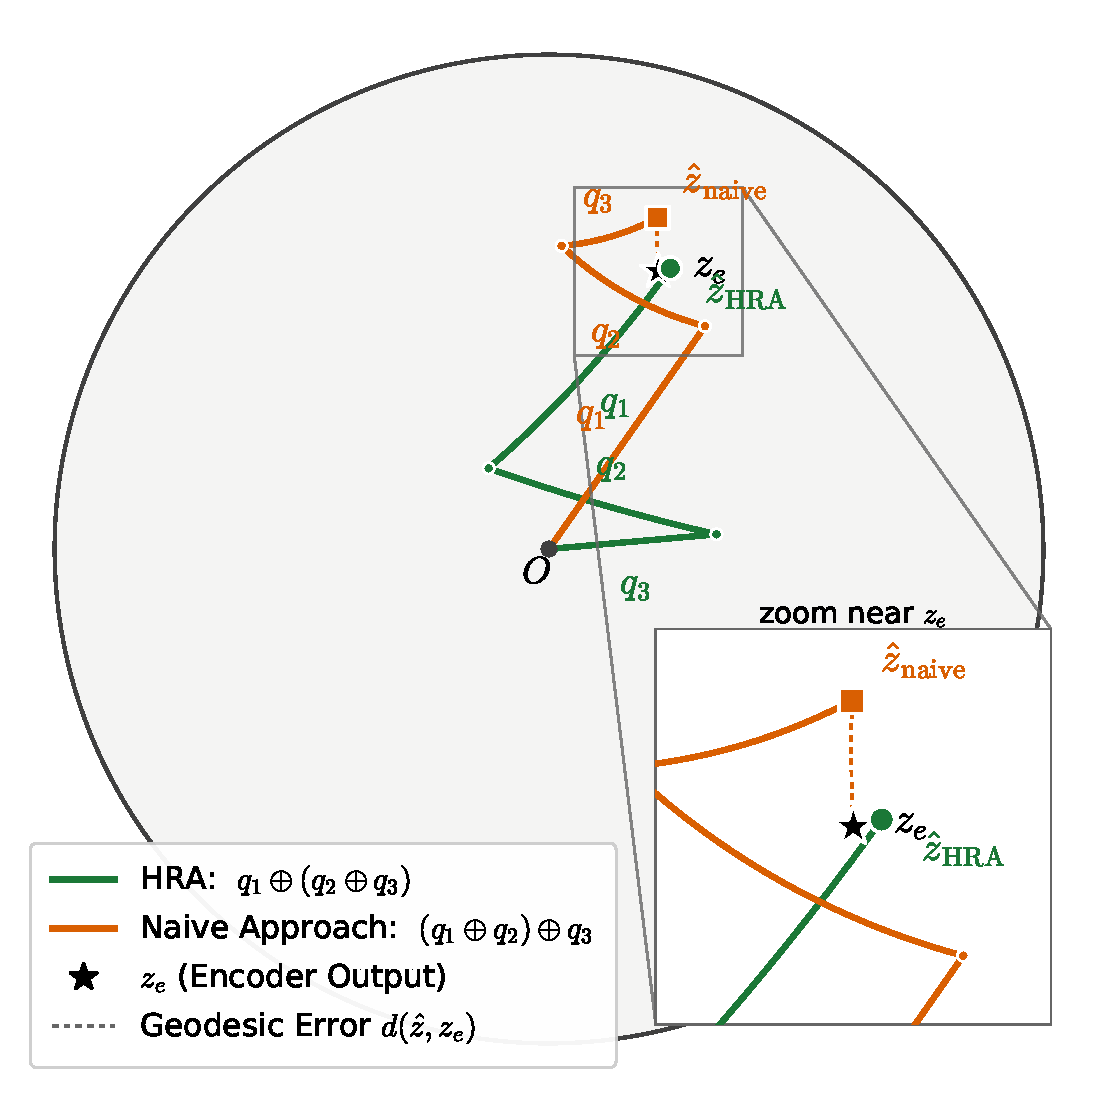
\includegraphics[width=0.78\textwidth]{../figures/poincare_aggregation}
    \caption{Residual aggregation of the same codewords under the two conventions of \S\ref{sec:residagg}, on the Poincar\'e disk ($c=1$, $N=3$). A single encoder point $z_e$ is residual-quantized into coarse-to-fine codes $q_1,q_2,q_3$ (a dominant $q_1$ oriented toward $z_e$ followed by progressively smaller refinements of the shrinking residual); each aggregation is drawn as the chain of M\"obius hops from the origin $O$ that sums these gyrovectors. The HRA reverse-nested order $q_1\oplus_c(q_2\oplus_c q_3)$ (green) inverts the left-subtraction recursion (Eq.~\ref{eq:hrq_residual}) and reaches $\hat z_{\mathrm{new}}$, which coincides with $z_e$ up to the final residual ($d=0.08$). The previous-work left-associated order $(q_1\oplus_c q_2)\oplus_c q_3$ (orange, Eq.~\ref{eq:prev_residual}) misplaces the gyration factors and drifts to $\hat z_{\mathrm{prev}}$ ($d=0.38$); the inset zooms on $z_e$. The instance is illustrative: $z_e$ is placed at moderate radius so the gap is legible. The drift is small for shallow, well-quantized residuals---where both orders nearly agree---and compounds with depth and proximity to the ball boundary, as analysed in \S\ref{sec:hrq}.}
    \label{fig:residagg}
\end{figure}

\chapter{Experimental Setup}
\label{chap:expsetup}

The methodology of Chapter~\ref{chap:methods} is geometry- and architecture-agnostic: it specifies how a residual quantizer routes gradients and aggregates codes on the Poincar\'e ball, independently of what the encoder and decoder are or what they encode. To test whether the hyperbolic treatment buys anything over a Euclidean residual quantizer, and whether the block-level estimator of \S\ref{sec:blockste} is what makes the difference, we evaluate the same quantizer in four settings that differ in modality, hierarchy, and stack depth: image reconstruction and generation (MNIST, CIFAR-100), language hierarchy embedding (WordNet), sequential recommendation (Amazon Reviews), and neural audio coding (LibriTTS at 24\,kHz). The four tasks span the shallow regime in which prior hyperbolic residual quantizers reported their results ($n_q=4$) and the deep regime in which the leaked-firewall pathology of \S\ref{sec:firewall} becomes decisive ($n_q=12$).

Across every task the experimental variable is the quantizer alone. The encoder, decoder, optimizer, data pipeline, and evaluation protocol are held fixed within a task, and we swap only the curvature and the straight-through/aggregation flags that select one of three configurations: a Euclidean RVQ baseline, the vanilla hyperbolic quantizer (the naive lift of \S\ref{sec:firewall}), and the block-level estimator with the Riemannian discount and gradient correction (the \emph{A4} configuration of \S\ref{sec:blockste}). These three are defined in \S\ref{sec:configs}; the tasks, datasets, architectures, hyperparameters, and metrics follow in \S\ref{sec:tasks}--\S\ref{sec:metrics}. All experiments run on a SLURM-managed HPC cluster (NVIDIA A100/H100 GPUs); the full code is available online.\footnote{\url{https://github.com/Sland0r/VAEs}}

\section{Compared Quantizer Configurations}
\label{sec:configs}

Every result in this thesis compares the same three quantizer configurations, isolated so that they differ only in the geometry and the gradient routing of \S\ref{sec:hste}, never in capacity. All three use the same number of residual stages $n_q$, the same codebook size, and the same encoder/decoder for a given task; they are selected entirely through command-line flags.

\paragraph{Euclidean (baseline).} Standard residual vector quantization (\,$c=0$\,) with the identity straight-through estimator and the additive residual recursion $r_i = r_{i-1}-q_i$, $\hat z=\sum_i q_i$ of \S\ref{sec:bg_rvq}. This is the reference point: any hyperbolic gain must be measured against it.

\paragraph{Vanilla hyperbolic.} The naive lift of \S\ref{sec:firewall} (\,$c=1$\,): the codebooks live on the Poincar\'e ball and assignment uses the squared geodesic distance, but the estimator keeps the Euclidean identity STE and the previous-work M\"obius transliteration (Eq.~\ref{eq:prev_residual}). This configuration carries both failures of \S\ref{sec:firewall} --- the copied gradient is geometrically wrong, and the residual firewall leaks --- and stands in for the recipe used by prior hyperbolic residual-quantization work~\cite{hrqvae}.

\paragraph{A4 (block-level estimator).} The estimator developed in \S\ref{sec:blockste} (\,$c=1$\,): the Hyperbolic Residual Aggregation (HRA) convention of \S\ref{sec:newmethod} (Eq.~\ref{eq:hrq_residual}, selected by \texttt{new\_method}), the block-level PT-STE (\texttt{block\_hste\_pt}) that transports a single aggregate gradient to the encoder, the discounted HSTE (d-HSTE, \texttt{hste\_riemannian}) of Eq.~\ref{eq:hste_riemannian}, and the residual gradient correction (\texttt{gradient\_correction}) of \S\ref{sec:firewall}. We refer to this combination as \emph{A4}, and to the gradient-corrected variant used throughout the deep-stack comparisons as \emph{A4\,+\,gc}.

The flag mapping is summarized in Table~\ref{tab:configs}. (A diagnostic-only flag, \texttt{--approx}, which tracks the hyperbolic approximation error without altering the model, is enabled in the hyperbolic runs and has no effect on the trained quantizer.) On the audio codec, whose $n_q=12$ stack pushes embeddings toward the ball boundary, the A4 configuration additionally activates the boundary controls discussed in \S\ref{sec:tasks_audio} (\texttt{--code\_max\_radius 0.9}, \texttt{--tangent\_proj}, \texttt{--encoder\_scale -1}, and \texttt{--uniform} quantizer-depth dropout); these are stabilizers, not changes to the estimator.

\begin{table}[h]
\centering
\caption{The three quantizer configurations compared throughout, with the command-line flags that select them. All other settings (stages, codebook size, encoder/decoder, optimizer) are held fixed within a task.}
\label{tab:configs}
\begin{tabular}{lcl}
\hline
Configuration & $c$ & Flags \\
\hline
Euclidean & $0$ & \emph{(none)} \\
Vanilla hyperbolic & $1$ & \emph{(default hyperbolic STE)} \\
A4 (block-level) & $1$ & \texttt{new\_method block\_hste\_pt hste\_riemannian} \\
A4 + gc & $1$ & \texttt{\ \ + gradient\_correction} \\
\hline
\end{tabular}
\end{table}

\section{Tasks and Datasets}
\label{sec:tasks}

\subsection{Image reconstruction and generation}
\label{sec:tasks_image}
The image task uses two standard benchmarks: MNIST ($28\times28$ grayscale, $60{,}000$ training and $10{,}000$ test images) and CIFAR-100 ($32\times32$ RGB, $50{,}000$ training and $10{,}000$ test images). CIFAR-100 additionally carries a two-level label hierarchy --- $100$ fine classes grouped into $20$ coarse superclasses of five classes each --- which we exploit to test whether the quantized latent space recovers the taxonomy without ever seeing the superclass labels (\S\ref{sec:metrics}). Pixels are normalized to $[-1,1]$; no data augmentation is applied, so the only source of variation between configurations is the quantizer.

\subsection{Language hierarchy embedding}
\label{sec:tasks_nlp}
The language task embeds the WordNet noun hierarchy~\cite{nickel2017poincare}, comprising all $82{,}115$ noun synsets and their hypernymy (is-a) edges, extracted via NLTK. The encoder is trained contrastively with an InfoNCE objective: each positive hypernymy edge is contrasted against $50$ sampled negatives, with the full transitive closure used only to filter the negative sampler so that no true ancestor is ever drawn as a negative. We use the \emph{closure} split, the harder of the two evaluation protocols, in which held-out edges may be reconstructed only by composing transitive relations; a no-model graph-composition baseline already attains $\approx 80\%$ recall@10 on this split, and a global-popularity baseline $\approx 41\%$, which together frame the difficulty of the task.

\subsection{Sequential recommendation}
\label{sec:tasks_rec}
The recommendation task follows the semantic-ID paradigm~\cite{tiger}: each item is mapped to a tuple of discrete codes by the residual quantizer, and a sequence model then predicts the next item's code tuple from a user's interaction history. We use three categories of the Amazon Reviews 2014 corpus --- Beauty (the headline dataset), Sports \& Outdoors ($18{,}357$ items), and Toys \& Games ($11{,}924$ items) --- under the standard leave-one-out split. Item content is encoded once into $768$-dimensional sentence embeddings with a pretrained MPNet sentence-transformer; these frozen embeddings are the input the quantizer compresses into semantic IDs. A uniqueness tie-break token (\texttt{--dedup}) is appended so that items colliding on all $n_q$ codes remain distinguishable, as is standard in this setting.

\subsection{Neural audio coding}
\label{sec:tasks_audio}
The audio task is a SoundStream-style neural codec~\cite{soundstream,encodec} trained on the LibriTTS \texttt{train-clean-100} corpus (read English speech) resampled to $24$\,kHz. This is the deepest stack we consider: $n_q=12$ residual quantizers with $1024$ codes each, which drives intermediate residuals toward the ball boundary and makes it the decisive test of the depth pathology of \S\ref{sec:firewall}. Because the boundary is where the conformal factors of Eq.~\ref{eq:hste_backward} diverge, the hyperbolic codec requires the explicit boundary controls noted in \S\ref{sec:configs}: a maximum code radius of $0.9$, a tangent-space projection to a reduced codebook dimension ($64$ via \texttt{--tangent\_proj}), an encoder-scale control, and \texttt{--uniform} quantizer-depth dropout (without which all hyperbolic runs collapse). We report results at codebook dimension $64$ for $3$- and $10$-epoch budgets.

\section{Model Architectures}
\label{sec:models}

\paragraph{Image VQ-VAE.} A convolutional VQ-VAE~\cite{vqvae}. The encoder is a stack of strided $2$-D convolutions ($\text{in}\to32\to64\to128\to D$ channels) that downsamples the image by a factor of four, followed by residual vector quantization; the decoder mirrors it with transposed convolutions. The latent dimension is $D=128$ and the quantizer uses $n_q=4$ stages of $128$ codes each. For generation we train, on top of the frozen quantizer, an RQ-Transformer prior~\cite{lee2022rqvae} (spatial and depth transformers, $4$ layers each, $8$ heads, model dimension $256$) and sample $10{,}000$ images from it.

\paragraph{WordNet encoder.} A lightweight embedding network maps each synset to a $16$-dimensional vector that is projected onto the ball and residual-quantized ($n_q=4$, $128$ codes). Recall@10 is measured by a paper-faithful beam-search seq2seq that generates a concept's hypernym code tuples from its own, trained for $10$ epochs on the frozen codes.

\paragraph{Recommendation RQ-VAE and recommender.} The quantizer is an RQ-VAE~\cite{lee2022rqvae,hrqvae} with a $768\!\to\!512\!\to\!32$ MLP encoder (and mirrored decoder), $n_q=4$ stages of $128$ codes. The downstream recommender is an encoder--decoder Transformer (model dimension $384$, $6$ layers, $6$ heads, feed-forward $1024$, dropout $0.1$) that autoregressively generates the next item's semantic ID with beam search ($50$ beams, history length $20$).

\paragraph{Audio codec.} A SEANet convolutional encoder/decoder~\cite{soundstream,encodec} with a $12$-stage residual quantizer ($1024$ codes per stage). Training is adversarial, with a multi-scale STFT discriminator, a multi-period discriminator, and a multi-scale (waveform) discriminator, combined with reconstruction and feature-matching losses; the codebook commitment term is weighted heavily ($\lambda_{\text{com}}=1000$) and the discriminators are switched on after $500$ steps.

\section{Training and Hyperparameters}
\label{sec:hparams}

Hyperparameters were tuned on the Euclidean baseline and then frozen and reused for the hyperbolic configurations, so that the comparison does not favor the proposed method; only the geometry-specific quantities (curvature, manifold learning rate) are set separately for the hyperbolic runs. Across all tasks the Euclidean parameters are optimized with AdamW and the manifold (codebook) parameters, where present, with Riemannian Adam from \texttt{geoopt}. The image and audio runs additionally clip the quantizer and manifold gradients (to $0.05$ and $0.02$ respectively) to keep the curved updates stable near the boundary. Table~\ref{tab:hparams} collects the per-task settings; curvature is $c=1$ for the hyperbolic configurations and $c=0$ for the Euclidean baseline throughout.

The image and audio results are reported as mean\,$\pm$\,std over three seeds ($42,43,44$); the image generation, language, and recommendation numbers are single-seed (a full re-run of the language capacity grid reproduced the reported numbers exactly, so no variance table is added there).

\begin{table}[h]
\centering
\caption{Per-task training configuration. ``Quantizer'' lists the residual depth $n_q$, the codebook size per stage, and the embedding dimension fed to the quantizer. Learning rate is the base (Euclidean-parameter) rate; manifold codebooks use a separate Riemannian-Adam rate.}
\label{tab:hparams}
\begin{tabular}{lcccc}
\hline
 & Image & Language & Recommendation & Audio \\
\hline
Dataset & MNIST/CIFAR-100 & WordNet & Amazon Reviews & LibriTTS 24\,kHz \\
Quantizer ($n_q$/bins/dim) & $4$/$128$/$128$ & $4$/$128$/$16$ & $4$/$128$/$32$ & $12$/$1024$/$64$ \\
Epochs & $50$ & $50$ & $5000$ & $3$--$10$ \\
Batch size & $128$ & $1024$ & $2048$ & $2$ (per GPU, DDP) \\
Base LR & $3\!\times\!10^{-4}$ & $1.0$ & $1\!\times\!10^{-4}$ & $3\!\times\!10^{-4}$ \\
Optimizer & AdamW\,+\,RAdam & RAdam & AdamW\,+\,RAdam & AdamW\,+\,RAdam \\
Commitment weight & $0.25$ & $1.0$ & $0.01$ & $1000$ \\
Seeds & $42,43,44$ & $42$ & $42$ & $42,43,44$ \\
\hline
\end{tabular}
\end{table}

\section{Evaluation Metrics}
\label{sec:metrics}

Each task is judged on the criterion that matters for it, and --- where the dataset permits --- on a separate measure of whether the learned code space is hierarchically organized, since reconstruction fidelity and hierarchical structure need not coincide.

\paragraph{Image.} Reconstruction is the best validation reconstruction loss (mean squared error). Generation quality is the Fr\'echet Inception Distance (FID, lower is better) and Inception Score (IS, higher is better) computed on $10{,}000$ RQ-Transformer samples with \texttt{torchmetrics}. Hierarchy recovery is measured on CIFAR-100 by treating each fine class's mean code embedding as a point and asking whether the $20$ superclasses re-emerge: we report sibling precision@4 (the fraction of a class's four nearest neighbours sharing its superclass), the ARI, NMI, and purity of an agglomerative clustering into $20$ groups, and the cophenetic correlation of the induced dendrogram against the ground-truth two-level tree (\texttt{scipy}/\texttt{scikit-learn}). No superclass labels are used in training.

\paragraph{Language.} Recall@10 for hypernymy reconstruction on the closure split, via beam-search generation. We additionally characterize representation quality through code-tuple statistics over all $82{,}115$ synsets: the uniqueness ratio (distinct code sequences per concept) and the intra-cluster semantic coherence of concepts that share a code, measured with WordNet path and Wu--Palmer tree similarity and GloVe embedding cosine.

\paragraph{Recommendation.} Top-$k$ ranking quality on the held-out item, reported as Recall@5/@10 and NDCG@5/@10, together with the pre-deduplication uniqueness ratio of the generated semantic IDs as a codebook-health diagnostic.

\paragraph{Audio.} The primary metric is the best validation reconstruction loss; codebook health is read from the per-layer validation perplexity across the $12$ stages (a collapse manifests as perplexity $\approx 1$ in all layers). We also report perceptual rate--distortion behaviour (PESQ, STOI, SI-SDR against entropy-estimated kbps).

\section{Implementation and Tools}
\label{sec:tools}

All models are implemented in PyTorch. The Poincar\'e-ball operations at the core of the quantizer --- the exponential and logarithmic maps, M\"obius addition, geodesic distance, gyration, and the projection that keeps points inside the ball --- are implemented from scratch (with the cancellation-free gyration of Appendix~\ref{app:gyration}), while \texttt{geoopt} supplies the manifold parameters and the Riemannian Adam optimizer used for the codebooks. WordNet access is through NLTK; the recommendation item embeddings are produced with a pretrained MPNet sentence-transformer; FID/IS are computed with \texttt{torchmetrics}, and the hierarchy-clustering metrics with \texttt{scipy} and \texttt{scikit-learn}. The audio codec is trained with distributed data parallelism across multiple GPUs; all other tasks run on a single GPU. Experiments are launched as SLURM batch jobs on the cluster described above.

\chapter{Experiments}
\label{chap:experiments}

We now put the three quantizer configurations of \S\ref{sec:configs} --- the Euclidean baseline, the vanilla hyperbolic lift of \S\ref{sec:firewall}, and the block-level A4 estimator of \S\ref{sec:blockste} --- to work on the four tasks of \S\ref{sec:tasks}. The chapter is organized to answer three questions in turn, each of which the geometry of Chapter~\ref{chap:methods} makes a concrete prediction about. \emph{First}, does hyperbolic curvature help when the data carries a latent hierarchy, and does it hurt when it does not? \emph{Second}, does the block-level estimator earn its keep --- i.e.\ does the depth pathology of \S\ref{sec:firewall} actually bite the vanilla lift, and does A4 contain it? \emph{Third}, does the HRA aggregation of \S\ref{sec:newmethod} reconstruct the encoder point on the ball as the telescoping argument claims? The four tasks are ordered by stack depth so that the shallow regime ($n_q=4$: images, language, recommendation) and the deep regime ($n_q=12$: audio) can be read against each other, since several of the geometry's effects are depth-conditional.

Throughout, the comparison is held to the three configurations of Table~\ref{tab:configs}; the many single-flag ablations we ran (per-layer HSTE, alternative residual routers, strict gradient-firewall variants) are not central to the three questions above and are deferred to Appendix~\ref{app:gc_leak} where they bear on the leaked-gradient analysis. On images and audio A4 includes the gradient correction (\emph{A4\,+\,gc}); on the shallow language and recommendation stacks the correction starves the commitment signal and is omitted, as anticipated in \S\ref{sec:configs} --- we flag the exception explicitly wherever it matters and report the gc ablation where it is informative (the audio dimension sweep, \S\ref{sec:exp_audio}).

\section{Image Reconstruction, Hierarchy, and Generation}
\label{sec:exp_image}

The image task is the cleanest separation of the three things a quantizer can be asked to do, because the same trained codes are scored three ways: as a compressor (reconstruction MSE), as a generative tokenizer (RQ-Transformer FID/IS), and --- on CIFAR-100, whose $100$ classes nest into $20$ superclasses --- as an unsupervised taxonomy (\S\ref{sec:metrics}). Tables~\ref{tab:img_recon}--\ref{tab:img_gen} report all three.

\begin{table}[h]
\centering
\caption{Image reconstruction. Best validation reconstruction loss ($\times10^{-3}$, lower is better), mean\,$\pm$\,std over seeds $42/43/44$. Euclidean wins both datasets.}
\label{tab:img_recon}
\begin{tabular}{lcc}
\hline
Configuration & MNIST & CIFAR-100 \\
\hline
Euclidean & $\mathbf{0.477 \pm 0.006}$ & $\mathbf{1.077 \pm 0.006}$ \\
Vanilla hyperbolic & $0.600 \pm 0.020$ & $1.280 \pm 0.017$ \\
A4 (block-level, +gc) & $0.647 \pm 0.023$ & $1.360 \pm 0.046$ \\
\hline
\end{tabular}
\end{table}

\begin{table}[h]
\centering
\caption{CIFAR-100 superclass hierarchy recovery (higher is better), mean\,$\pm$\,std over seeds $42/43/44$. No superclass labels are seen in training. A4 leads the clustering metrics (ARI, NMI, purity); vanilla edges sibling precision and cophenetic correlation.}
\label{tab:img_hier}
\begin{tabular}{lccccc}
\hline
Configuration & prec@4 & ARI & NMI & purity & coph.\ corr \\
\hline
Euclidean & $0.159 \pm 0.001$ & $0.048 \pm 0.005$ & $0.469 \pm 0.012$ & $0.327 \pm 0.006$ & $0.046 \pm 0.001$ \\
Vanilla hyperbolic & $\mathbf{0.164 \pm 0.003}$ & $0.055 \pm 0.003$ & $0.481 \pm 0.003$ & $0.337 \pm 0.006$ & $\mathbf{0.052 \pm 0.002}$ \\
A4 (+gc) & $0.157 \pm 0.004$ & $\mathbf{0.087 \pm 0.008}$ & $\mathbf{0.515 \pm 0.013}$ & $\mathbf{0.370 \pm 0.010}$ & $0.043 \pm 0.005$ \\
\hline
\end{tabular}
\end{table}

\begin{table}[h]
\centering
\caption{Image generation. RQ-Transformer, $10{,}000$ samples, single seed: FID (lower is better) with Inception Score in parentheses (higher is better). Note the dataset reversal --- every hyperbolic variant beats Euclidean on MNIST, while Euclidean wins CIFAR.}
\label{tab:img_gen}
\begin{tabular}{lcc}
\hline
Configuration & MNIST FID (IS) & CIFAR-100 FID (IS) \\
\hline
Euclidean & $20.36\ (2.069)$ & $\mathbf{94.67}\ (3.86)$ \\
Vanilla hyperbolic & $\mathbf{15.01}\ (2.105)$ & $101.84\ (3.51)$ \\
A4 (+gc) & $16.78\ (2.068)$ & $98.23\ (3.80)$ \\
\hline
\end{tabular}
\end{table}

\paragraph{A three-way dissociation.} The striking finding is that the ranking of the three configurations \emph{changes with the criterion}. As a pure compressor (Table~\ref{tab:img_recon}) Euclidean is best on both datasets and the hyperbolic configurations trail by $25$--$30\%$ relative MSE, with A4 slightly behind vanilla --- consistent with the prediction of \S\ref{sec:blockste} that the curved estimator buys gradient correctness, not distortion. On hierarchy recovery (Table~\ref{tab:img_hier}) the order inverts on the metrics that measure global tree structure: A4 lifts ARI from the Euclidean $0.048$ to $0.087$ ($+80\%$) and leads NMI and purity, with every hyperbolic configuration above Euclidean --- exactly the behaviour the hyperbolic hypothesis predicts for data with a latent taxonomy. Sibling precision@4 separates almost nothing (all rows $0.157$--$0.164$), and the cophenetic correlation slightly favours vanilla; the clustering metrics, which read the coarse $20$-way grouping rather than the local $4$-nearest-neighbour structure, are where the geometry shows up. On generation (Table~\ref{tab:img_gen}) the picture splits by dataset: on MNIST every hyperbolic configuration beats Euclidean (vanilla best, FID $15.0$ vs $20.4$, $-26\%$), so hyperbolic codes are better autoregressive tokens \emph{even though they are worse reconstructions}; on CIFAR Euclidean takes FID, with A4 the best of the hyperbolic arms.

\paragraph{Reading.} No single configuration dominates, and that is the point: reconstruction fidelity, generative token quality, and hierarchical organization of the code space are genuinely different objectives, and curvature trades the first for the latter two on data that has a hierarchy to recover. The narrow spread of every generation and hierarchy column is itself informative --- it is consistent with the codes sitting near an information ceiling, so that the quantizer geometry reorganizes \emph{how} the fixed bit budget is spent (toward taxonomy and toward better next-token statistics) rather than how much information the codes carry.

\section{Language Hierarchy Embedding}
\label{sec:exp_nlp}

WordNet is the task with the most explicit ground-truth hierarchy, and therefore the sharpest test of the central hypothesis. We report the closure split (\S\ref{sec:tasks_nlp}), against which a no-model graph-composition baseline already reaches $\approx 80\%$ recall@10 and a global-popularity baseline $\approx 41\%$; these frame what a learned code space must beat to have learned anything transferable. Table~\ref{tab:nlp_grid} sweeps the embedding dimension and codebook size around the standard $d{=}16,\ \text{bins}{=}128$ cell.

\begin{table}[h]
\centering
\caption{WordNet hierarchy, Recall@10 (\%) on the closure split, single seed. Capacity grid over embedding dimension and codebook size; the $d16/b128$ column is the standard configuration. Best per column in bold. A4 here is the shallow-depth (no-gc) configuration of \S\ref{sec:configs}.}
\label{tab:nlp_grid}
\resizebox{\textwidth}{!}{%
\begin{tabular}{lccccccc}
\hline
Configuration & $d8/b128$ & $d8/b256$ & $d16/b64$ & $d16/b128$ & $d16/b256$ & $d32/b128$ & $d32/b256$ \\
\hline
Euclidean & $\mathbf{75.4}$ & $\mathbf{63.4}$ & $76.7$ & $75.9$ & $67.0$ & $\mathbf{71.1}$ & $51.9$ \\
Vanilla hyperbolic & $62.3$ & $42.6$ & $\mathbf{86.9}$ & $83.4$ & $\mathbf{81.7}$ & $53.6$ & $\mathbf{65.2}$ \\
A4 (no gc) & $61.6$ & $39.7$ & $82.3$ & $\mathbf{84.1}$ & $81.6$ & $36.6$ & $40.2$ \\
\hline
\end{tabular}}
\end{table}

\paragraph{Hyperbolic owns the trainable sweet spot.} In the $d16$ band --- the regime the encoder actually trains cleanly in --- hyperbolic wins decisively at every codebook size: vanilla $86.9$ and A4 $84.1$ against Euclidean's $75.9$ at the standard cell, a $+8$--$11$ point gap, with the within-hyperbolic winner shifting from vanilla at the small book ($d16/b64$) to A4 at the standard/large book ($d16/b128$). Euclidean leads only in the two \emph{broken} regimes, and the failures there have opposite causes, both verified from training diagnostics. The $d32$ columns are an init/boundary collapse specific to the hyperbolic runs: at the default initialization the embedding norm grows as $\sqrt{d}$ ($\approx 5.7$ at $d32$), the exponential map saturates against the ball boundary, the commitment distance hits its clamp, and the model barely trains --- the boundary pathology of \S\ref{sec:firewall}, here on the encoder side. (It is curative-by-initialization, not a capacity limit: a $\sqrt{d}$-compensated init restores these cells to the $80$s, but that lies outside the three-configuration comparison and we note it only to attribute the failure correctly.) The $d8/b256$ collapse is the reverse pathology --- codebook over-provisioning, not boundary saturation: the VAE trains cleanly but $256$ codes cannot be usefully spread across $8$ hyperbolic dimensions, so almost every concept receives a unique code tuple and the seq2seq memorizes rather than generalizes. Euclidean tolerates over-provisioning by spreading codes more widely and has no boundary to saturate, which is why it ``wins'' precisely the cells where the hyperbolic model is mistrained. Read against the baselines, the collapsed cells ($36$--$52$) sit at or below the $41\%$ popularity floor --- nothing transferable was learned --- while the winning $d16$ cells ($84$--$87$) close most of the gap to the $80\%$ composition ceiling and clear it outright.

\begin{table}[h]
\centering
\caption{WordNet representation quality at the standard cell ($d16/b128$), over all $82{,}115$ noun synsets. Uniqueness = distinct code sequences per concept (and number of clusters where $>1$ concept shares a code). Similarity columns: WordNet path and Wu--Palmer tree similarity and GloVe cosine of concepts sharing a code (higher = tighter group).}
\label{tab:nlp_repr}
\begin{tabular}{lcccccc}
\hline
Configuration & uniq.\ ratio & clusters $>1$ & max cluster & path sim & wup sim & GloVe sim \\
\hline
Euclidean & $0.997$ & $32$ & $163$ & $0.123$ & $0.320$ & $0.336$ \\
Vanilla hyperbolic & $0.888$ & $6486$ & $582$ & $0.078$ & $0.242$ & $0.097$ \\
A4 (+gc) & $0.967$ & $2161$ & $456$ & $0.088$ & $0.262$ & $0.162$ \\
\hline
\end{tabular}
\end{table}

\paragraph{What the codes cluster (and a confound).} Table~\ref{tab:nlp_repr} asks not how well the codes retrieve hypernyms but how they organize the vocabulary. Read naively the similarity columns favour Euclidean, but that is an artifact of its barely clustering at all: it is near-injective ($99.7\%$ unique codes, only $32$ genuine collisions), using the codebook as a hash rather than a shared structure, so averaging similarity over its handful of accidental near-synonym collisions trivially looks coherent --- averaging intra-cluster similarity structurally rewards \emph{not} clustering. The meaningful comparison is between the two configurations that actually cluster, and there \textbf{A4 beats vanilla on both axes}: it is more selective (uniqueness $0.967$ vs $0.888$, i.e.\ $2161$ vs $6486$ clusters --- it does not over-collapse the codebook) \emph{and} more semantically coherent on all three similarity measures (path $0.088$ vs $0.078$, Wu--Palmer $0.262$ vs $0.242$, GloVe $0.162$ vs $0.097$). Vanilla over-clusters into looser groups; A4's tighter, more coherent clusters are the representation-quality counterpart of its hierarchy win on CIFAR. (The honest caveat: comparing average pairwise similarity across very different cluster counts is apples-to-oranges, and a fully rigorous version would report lift over a random-code baseline --- expected $\approx 0$ for the near-injective Euclidean codes, positive for the hyperbolic ones.)

\section{Sequential Recommendation}
\label{sec:exp_rec}

The recommendation task tests whether the same code-space organization helps a genuinely downstream objective: semantic IDs generated once by the quantizer are consumed by a seq2seq recommender (\S\ref{sec:tasks_rec}). We report the Beauty category; the two further Amazon categories we ran are excluded here pending a clean rerun.\footnote{The Sports \& Outdoors and Toys \& Games runs are omitted because their recommender stage was affected by a code-file naming inconsistency; only Beauty is reported until they are rerun cleanly.}

\begin{table}[h]
\centering
\caption{Amazon Beauty, test-set ranking metrics (higher is better) and the pre-deduplication uniqueness ratio as a codebook-health diagnostic. A4 here is the +gc configuration; the no-gc variant is within noise of it ($0.970$ uniq., R@5 $0.0398$, R@10 $0.0591$). Best per column in bold.}
\label{tab:rec_beauty}
\begin{tabular}{lccccc}
\hline
Configuration & uniq.\ ratio & R@5 & NDCG@5 & R@10 & NDCG@10 \\
\hline
Euclidean$^\ast$ & $0.932$ & $0.0342$ & $0.0235$ & $0.0513$ & $0.0290$ \\
Vanilla hyperbolic & $0.872$ & $0.0388$ & $0.0250$ & $0.0600$ & $0.0318$ \\
A4 (+gc) & $\mathbf{0.973}$ & $\mathbf{0.0393}$ & $\mathbf{0.0259}$ & $\mathbf{0.0611}$ & $\mathbf{0.0329}$ \\
\hline
\end{tabular}
\end{table}

{\small $^\ast$The Euclidean baseline is not strictly matched --- it ran without the deduplication token and at a smaller batch --- so its absolute numbers are a lower bound and a matched rerun is pending; the hyperbolic gap is large enough that the conclusion is unlikely to reverse.}

\paragraph{Reading.} Both hyperbolic configurations beat Euclidean on every metric. The mechanism is visible in the uniqueness column: A4 restores codebook health (uniqueness $0.973$) where vanilla under-uses the codebook ($0.872$), and the healthier codebook turns into better recommendations across the board (R@10 $0.0611$ vs Euclidean $0.0513$, $+19\%$). Consistent with the shallow-depth story of \S\ref{sec:exp_nlp}, the gradient correction barely moves anything at $n_q=4$ (the no-gc variant is a near-tie with the +gc row reported here): the deep-stack machinery that A4 adds over vanilla has little to fix on a four-stage recommender, and its contribution here is the codebook-health repair, not the depth fix.

\section{Neural Audio Coding}
\label{sec:exp_audio}

Audio is the deep-stack task --- $n_q=12$ residual quantizers of $1024$ codes each --- and therefore the decisive test of the depth pathology of \S\ref{sec:firewall} and of whether the block-level estimator contains it. It is also, deliberately, the task with \emph{no} latent hierarchy to exploit, so it isolates the quantizer purely as a compressor. The hyperbolic codec requires the boundary controls of \S\ref{sec:tasks_audio} (a maximum code radius, the tangent-space projection to dimension $64$, the encoder-scale control, and \texttt{--uniform} quantizer-depth dropout); without \texttt{--uniform} \emph{every} hyperbolic run collapses, so it is a precondition rather than a tuned option.

\begin{table}[h]
\centering
\caption{SoundStream 24\,kHz, $n_q=12$, codebook dimension $64$. Best validation reconstruction loss (lower is better); codebook health is the per-layer validation perplexity across the $12$ stages (collapse $=$ perplexity $\approx 1$). Vanilla hyperbolic has no healthy $10$-epoch checkpoint.}
\label{tab:audio_d64}
\begin{tabular}{lccc}
\hline
& \multicolumn{2}{c}{val.\ recon $\downarrow$} & \\
Configuration & $3$ epochs & $10$ epochs & codebook health ($3$ ep) \\
\hline
Euclidean & $179.73$ & $\mathbf{117.63}$ & all $12$ alive, $625$--$871$ \\
Vanilla hyperbolic & $211.99$ & --- & all alive (degraded) \\
A4 (riem\,+\,gc) & $\mathbf{177.72}$ & $121.18$ & all $12$ alive, $101$--$513$ \\
\hline
\end{tabular}
\end{table}

\begin{table}[h]
\centering
\caption{Audio dimension-sweep viability envelope (A4, $3$ epochs, val.\ recon $\downarrow$). The gradient correction is \emph{required} at dimension $64$ but \emph{fatal} at dimensions $8$ and $128$ and at native dimension; A4's viable envelope is $d32$--$d64$ only. $\boldsymbol{\times}$ marks codebook collapse.}
\label{tab:audio_dim}
\begin{tabular}{lccc}
\hline
dim & Euclidean & A4 (+gc) & A4 (no gc) \\
\hline
$8$   & $160.6$ & $265.9\ \boldsymbol{\times}$ & $263.3\ \boldsymbol{\times}$ \\
$32$  & $157.1$ & $179.0$ & $183.0$ \\
$64$  & $179.7$ & $\mathbf{177.7}$ & $264.7\ \boldsymbol{\times}$ \\
$128$ & $159.7$ & $279.9\ \boldsymbol{\times}$ & $261.3\ \boldsymbol{\times}$ \\
\hline
\end{tabular}
\end{table}

\paragraph{The depth pathology bites, and A4 contains it.} The vanilla lift is exactly where \S\ref{sec:firewall} predicts it will struggle: at $n_q=12$ it reconstructs at $211.99$, worse than Euclidean's $179.73$ and well behind A4 --- the accumulated leak of Eq.~\ref{eq:stack} has turned from signal into noise over twelve composed stages. A4, which routes a single transported gradient to the encoder instead (Eq.~\ref{eq:block_hste}), recovers a healthy codebook (all $12$ layers alive) and reaches $177.72$ at $3$ epochs --- marginally ahead of Euclidean and a full $34$ points ahead of vanilla. This is the clearest demonstration in the thesis that the block-level estimator is what makes the deep hyperbolic stack trainable at all: the difference between vanilla and A4 here is precisely the difference between the leaky per-stage routing of \S\ref{sec:firewall} and the single-hop routing of \S\ref{sec:blockste}.

\paragraph{But hyperbolic is not a better compressor.} The advantage does not survive more training or more bottleneck width. At $10$ epochs Euclidean retakes the lead ($117.63$ vs A4's $121.18$), and the dimension sweep (Table~\ref{tab:audio_dim}) shows Euclidean healthy at every width while A4 is viable only in a narrow $d32$--$d64$ envelope. The gradient correction is sharply non-monotone in dimension: required to keep $d64$ alive (without it, $d64$ collapses), yet fatal at $d8$, $d128$, and native dimension --- the same gc sign-flip seen across depth in the other tasks. Perceptual rate--distortion is flat for the hyperbolic codec (adding stages adds bits, not quality). On a task with no hierarchy to recover, the honest summary is that the hyperbolic codec's whole contribution is collapse-avoidance: A4 makes a deep curved stack \emph{trainable}, but trainability buys parity-at-best against a Euclidean codec that never had the problem in the first place.

\section{Residual Reconstruction Error Across Tasks}
\label{sec:exp_approx}

The final experiment is a direct check of the geometric claim of \S\ref{sec:newmethod}: that the HRA ordering makes the residual cascade telescope, so the codes recompose to the encoder point on the ball, whereas the previous-work transliteration (Eq.~\ref{eq:prev_residual}) drifts. The diagnostic \texttt{--approx} flag logs the squared hyperbolic distance between the quantizer's aggregate-plus-leftover and the encoder output --- zero iff reconstruction is exact on the ball. It is defined only for the hyperbolic configurations (Euclidean has no ball). Table~\ref{tab:approx} collects it across tasks; the block hop leaves the forward value unchanged, so these numbers are properties of the residual aggregation, not of the gradient estimator.

\begin{table}[h]
\centering
\caption{Mean validation residual on the ball (squared hyperbolic distance between the reconstructed code aggregate and the encoder output; lower is better, $0$ = exact). Vanilla uses the previous-work transliteration; A4 uses the HRA ordering. Recommendation is Beauty only; audio is recomputed at fixed full depth $n_q=12$.}
\label{tab:approx}
\begin{tabular}{llccc}
\hline
Task & Cell & Vanilla hyperbolic & A4 (+gc) & A4 (no gc) \\
\hline
Image  & MNIST            & $0.00049$ & $<\!10^{-5}$ & $<\!10^{-5}$ \\
Image  & CIFAR-100        & $0.00133$ & $<\!10^{-5}$ & $<\!10^{-5}$ \\
Rec    & Beauty           & $44.79$   & $0.031$ & $0.014$ \\
Audio  & $d64$, $3$ ep    & $57.77$   & $0.145$ & $57.77^{\dagger}$ \\
Audio  & $d64$, $10$ ep   & ---       & $0.026$ & --- \\
NLP    & $d16/b128$       & $\sim\!14.4$ & $12.9$ & $8.9$ \\
\hline
\end{tabular}
\end{table}

{\small $^{\dagger}$The A4-no-gc $d64/3$-ep cell is the collapsed run of Table~\ref{tab:audio_dim}: its reconstruction lands on the ball boundary, where the distance saturates at the same atanh-clamp ceiling ($\approx 57.77$) that any boundary-saturated model returns --- hence the exact match with vanilla, which is a collapse signature, not faithful reconstruction.}

\paragraph{Reading.} The prediction of \S\ref{sec:newmethod} holds in every domain. The HRA aggregation reconstructs the encoder point on the ball almost exactly --- A4's residual collapses toward zero, strikingly so in recommendation and audio ($0.01$--$0.15$ against vanilla's $45$--$58$) --- because the left-subtraction/reverse-nested pairing of Eq.~\ref{eq:hrq_residual} telescopes. The vanilla transliteration, by contrast, leaves a large residual: its per-stage M\"obius subtractions never invert the aggregation, so the cascade does not return the encoder point, exactly the mismatch analysed in \S\ref{sec:hrq}. NLP at $d16$ is the one regime where the two stay comparable ($\sim\!9$--$14$): at low curvature-scaled radius and shallow depth the gyration drift is small, as Figure~\ref{fig:residagg} anticipates. The two image cells are genuinely below $10^{-5}$, not missing data --- at the small radii reached on MNIST/CIFAR the telescoping is numerically exact.

\section{Summary}
\label{sec:exp_summary}

Read across the four tasks, the three questions of the chapter introduction get clear answers. \emph{(1) Hyperbolic captures hierarchy --- supported.} Where the data has a latent taxonomy, every hyperbolic configuration beats Euclidean: A4 lifts CIFAR-100 superclass ARI by $80\%$ (Table~\ref{tab:img_hier}), hyperbolic owns the trainable WordNet sweet spot by $8$--$11$ recall points (Table~\ref{tab:nlp_grid}), and the gains carry into downstream recommendation (Table~\ref{tab:rec_beauty}) and into MNIST generation, where hyperbolic codes are better autoregressive tokens despite being worse reconstructions (Table~\ref{tab:img_gen}). \emph{(2) The block-level estimator earns its keep at depth --- supported.} The vanilla lift degrades exactly where \S\ref{sec:firewall} predicts, on the $n_q=12$ audio stack ($211.99$ vs A4's $177.72$, Table~\ref{tab:audio_d64}), and A4's single-hop routing is what keeps the deep curved codebook alive. \emph{(3) The HRA aggregation telescopes --- supported.} Its on-ball reconstruction residual collapses to near-zero in every domain while the previous-work convention leaves a large drift (Table~\ref{tab:approx}). The one hypothesis the data does \emph{not} support is hyperbolic-as-pure-compressor: Euclidean wins reconstruction on all three image datasets and at audio scale, and A4's value on the hierarchy-free audio task reduces to collapse-avoidance. A4's defensible claim is therefore robustness and trainability --- it stays in a tight performance band across regimes that swing the vanilla lift from collapse to its best cells, and it is the only hyperbolic configuration that survives the deep stack --- while several of the headline absolute wins (the WordNet sweet-spot peak, the MNIST generation FID) belong to the plain vanilla quantizer once its boundary is controlled.

\chapter{Ablation Studies}
\label{ch:ablation}

The experiments of the previous chapter held the comparison to the three configurations of Table~\ref{tab:configs}, so that A4's contribution is read against a fixed reference. This chapter opens that comparison up. A4 is not a single switch but a particular choice of \emph{how reconstruction and commitment gradients are routed back to the encoder}; by perturbing one routing decision at a time --- always relative to A4 --- we isolate which channel actually carries the hyperbolic gain, and show that the winning choice is depth-conditional. WordNet, with its explicit ground truth and shallow $n_q=4$ stack, is the natural microscope and carries the bulk of the analysis; we then check whether the same routers transfer to the other three tasks.

\section{The encoder's gradient channels}
\label{sec:abl_channels}

The encoder maps a concept to a point $r_0=z_e$ on the ball; the residual quantizer turns it into a code tuple and a reconstruction, and during training the encoder receives gradient from up to four distinct routes.

\begin{itemize}
\item \textbf{Per-layer reconstruction ($R_{\text{layer}}$)} --- the reconstruction gradient flowing back through the \emph{attached} residual chain one stage at a time, i.e.\ the full sum of Eq.~\ref{eq:stack}. The vanilla lift and the per-layer d-HSTE keep it open; A4 closes it (the block straight-through detaches the per-layer codes).
\item \textbf{Block reconstruction hop ($R_{\text{block}}$)} --- the single block-level PT-STE of \S\ref{sec:blockste}, which transports one aggregate gradient to the encoder and nothing to the codes. A4 is defined by having only this recon route open.
\item \textbf{Commitment ($C$)} --- the term pulling the encoder toward its assigned codes. Its \emph{breadth} is itself a routing choice: all stages (no gc), the coarsest stage only (gc), the coarsest stage with the residual leak removed (strict gc), or off ($\text{commitment weight}=0$). The gc mechanism is analysed in Appendix~\ref{app:gc_leak}.
\item \textbf{Riemannian discount (riem)} --- the conformal $\lambda^2$ rescaling of the recon gradient (the d-HSTE of Eq.~\ref{eq:hste_riemannian}) that prevents the boundary blow-up of the naive estimator.
\end{itemize}

In these terms A4 is $\{R_{\text{layer}}$ off, $R_{\text{block}}$ on, $C$ on, riem on$\}$. The per-layer d-HSTE (which we label \emph{A3}: \texttt{new\_method hste hste\_riemannian}) is A4 with $R_{\text{block}}$ traded back for $R_{\text{layer}}$. The recon routers reopen restricted slices of $R_{\text{layer}}$: \emph{keep-first} (a6) and \emph{keep-last} (a7) route it through only the first or last stage on the A3 base, while their summed variants (a6.1, a7.1) and the un-truncated \emph{full-sum} router (a8) add the slice on top of A4's block hop.

\section{Gradient routing on WordNet}
\label{sec:abl_nlp}

Table~\ref{tab:abl_nlp} reports Recall@10 at the standard cell ($d16/b128$, $\text{cw}=1.0$, single seed) for the full routing family.

\begin{table}[h]
\centering
\caption{WordNet gradient-routing ablation, Recall@10 (\%) at the standard cell ($d16/b128$, closure split). All rows are perturbations of A4 along a single routing axis. a6/a7 are means of three seeds ($84.8$: $84.8/84.2/85.3$; $85.6$: $85.6/85.9/85.2$); strict gc is a mean of three ($75.2/75.5/75.2$). Euclidean ($75.9$) and the A4 reference are reproduced from Table~\ref{tab:nlp_grid}.}
\label{tab:abl_nlp}
\resizebox{\textwidth}{!}{%
\begin{tabular}{llc}
\hline
Configuration & Encoder recon routing & R@10 \\
\hline
Euclidean & per-layer (identity STE) & $75.9$ \\
Vanilla hyperbolic & per-layer (leaked) & $83.4$ \\
\quad + gc & per-layer, coarsest commit & $82.3$ \\
\hline
Per-layer d-HSTE (A3) & per-layer chain, no block hop & $85.2$ \\
\quad + gc & per-layer, coarsest commit & $81.5$ \\
A4 (no gc) & block hop, all commit & $84.1$ \\
\quad + gc & block hop, coarsest commit & $81.9$ \\
Strict gc (A4\,$v2$) & block hop, commit leak removed & $75.3$ \\
A5 (no gc) & block hop + last-commit chain & $84.4$ \\
\quad + gc & block hop + last-commit chain & $84.4$ \\
\hline
Keep-first router (a6) & first-stage recon (A3 base) & $84.8$ \\
Keep-last router (a7) & last-stage recon (A3 base) & $\mathbf{85.6}$ \\
a6.1 (A4 $\oplus$ a6) & block hop + first-stage recon & $84.6$ \\
a7.1 (A4 $\oplus$ a7) & block hop + last-stage recon & $85.0$ \\
Full-sum router (a8) & block hop + all per-layer recon & $\mathbf{85.6}$ \\
\hline
\end{tabular}}
\end{table}

\paragraph{At shallow depth the per-layer chain is the asset, not the block hop.} The top of the table is the per-layer family: keep-last (a7, $85.6$), the full-sum router (a8, $85.6$) and the plain per-layer d-HSTE (A3, $85.2$) lead, all ahead of the best pure block-hop arm (A4 no-gc, $84.1$). This inverts the audio verdict of \S\ref{sec:exp_audio} and is exactly what the depth argument predicts: at $n_q=4$ there is no compounding for the block hop to firewall, so reopening the per-layer reconstruction --- the full sum of Eq.~\ref{eq:stack} --- only adds signal. The full-sum router a8, which restores \emph{all} per-layer terms on top of A4's hop, recovers the per-layer ceiling exactly ($85.6$).

\paragraph{Commitment is the load-bearing channel.} Holding the block hop on and toggling the per-layer recon and commitment channels isolates where the gain lives (Table~\ref{tab:abl_isolate}). With the hop as the sole recon route, switching commitment on lifts the encoder from $74.7$ --- \emph{below} Euclidean --- to $81.8$; switching per-layer reconstruction on instead, with commitment off, barely moves it ($75.6$). The block hop alone carries almost no usable encoder signal at this depth; A4's performance is its commitment. This study runs at $\text{cw}=0.25$ rather than the $1.0$ of the rest of the chapter, because ``commitment off'' is intrinsically $\text{cw}=0$ and the comparison must share an operating point.

\begin{table}[h]
\centering
\caption{Channel isolation on WordNet ($d16/b128$, $\text{cw}=0.25$), block hop held on. Switching the commitment channel on or off, with and without the per-layer recon chain. Baselines at the same operating point: Euclidean $75.4$, vanilla $79.4$.}
\label{tab:abl_isolate}
\begin{tabular}{lc}
\hline
Routing (block hop always on) & R@10 \\
\hline
Block hop + all commit (A4 no gc) & $81.8$ \\
Block hop + per-layer recon, no commit (a8, cw$0$) & $75.6$ \\
Block hop only (no recon chain, no commit) & $74.7$ \\
\hline
\end{tabular}
\end{table}

\paragraph{The Riemannian discount is load-bearing only where transports compound.} The d-HSTE rescaling can be dropped independently (Table~\ref{tab:abl_riem}). For the per-layer family it is mandatory: A3 collapses from $85.2$ to $54.7$ without it, because the per-layer estimator applies $n_q$ compounding tangent transports and each amplifies the boundary $\lambda^2$ blow-up of \S\ref{sec:firewall}. The block hop, a single transport that never compounds, does not need it at all --- A4 is in fact marginally better without ($84.1\!\to\!84.7$). This is the routing-level reason A4 trades the per-layer chain for one block hop: it engineers away the very compounding that makes the discount necessary.

\begin{table}[h]
\centering
\caption{Riemannian discount ablation on WordNet ($d16/b128$, $\text{cw}=1.0$, no gc). Recall@10 with and without the d-HSTE $\lambda^2$ rescaling.}
\label{tab:abl_riem}
\begin{tabular}{lcc}
\hline
Family & discount on & discount off \\
\hline
Per-layer chain (A3) & $85.2$ & $54.7$ \\
Block hop (A4) & $84.1$ & $84.7$ \\
\hline
\end{tabular}
\end{table}

\paragraph{The commit firewall is monotone here.} Reading down the commitment-breadth rows of Table~\ref{tab:abl_nlp}, every commit path closed costs Recall: all-stage ($84.1$) $\to$ coarsest-only gc ($81.9$) $\to$ leak-removed strict gc ($75.3$, a full collapse to the Euclidean level). Removing even the residual \emph{leak} that plain gc still passes through --- the term analysed in Appendix~\ref{app:gc_leak} --- starves the encoder entirely, confirming from the destructive side that the leaked coarse-stage commitment is what the shallow stack runs on. This is the opposite of the deep-stack regime, where gc is the firewall that prevents collapse (\S\ref{sec:exp_audio}); the sign of gc's effect flips with depth.

\section{Routers and the strict firewall across tasks}
\label{sec:abl_crosstask}

The WordNet routers transfer to the other tasks unevenly, and the pattern is again depth. Table~\ref{tab:abl_rec} runs them on Amazon Beauty ($n_q=4$).

\begin{table}[h]
\centering
\caption{Gradient-routing ablation on Amazon Beauty (test set, $n_q=4$). The A4 reference is reproduced from Table~\ref{tab:rec_beauty}. Uniqueness is the pre-deduplication codebook-health diagnostic.}
\label{tab:abl_rec}
\begin{tabular}{lccccc}
\hline
Configuration & uniq.\ ratio & R@5 & NDCG@5 & R@10 & NDCG@10 \\
\hline
A4 (+gc), reference & $0.973$ & $0.0393$ & $0.0259$ & $\mathbf{0.0611}$ & $0.0329$ \\
A5 (+ last-commit chain) & $0.974$ & $\mathbf{0.0399}$ & $\mathbf{0.0276}$ & $0.0585$ & $\mathbf{0.0335}$ \\
Keep-first router (a6) & $0.970$ & $0.0372$ & $0.0251$ & $0.0567$ & $0.0314$ \\
Keep-last router (a7) & $0.975$ & $0.0381$ & $0.0251$ & $0.0588$ & $0.0317$ \\
Full-sum router (a8) & $0.973$ & $0.0395$ & $0.0267$ & $0.0601$ & $0.0333$ \\
Strict gc (A4\,$v2$) & $0.208$ & $0.0327$ & $0.0229$ & $0.0490$ & $0.0281$ \\
\hline
\end{tabular}
\end{table}

\paragraph{Shallow recommendation echoes WordNet.} The two strongest new arms are the ones that add commitment or reconstruction breadth on top of A4: the last-commit chain A5 tops the @5 metrics and NDCG@10 ($0.0399/0.0276/0.0335$), and the full-sum router a8 is a close second ($0.0395/0.0267/0.0333$), with A4 retaining the R@10 lead ($0.0611$). The per-layer-only routers a6/a7 land at or just below A4 while keeping the codebook healthy (uniqueness $\sim\!0.97$). Strict gc, by contrast, \emph{collapses} the codebook (uniqueness $0.208$) and drops below the Euclidean baseline (R@10 $0.0490 < 0.0513$), the same firewall-starvation failure seen on WordNet ($75.3$) --- confirming across a third task that the coarse-stage commitment leak is load-bearing.

\paragraph{At depth the per-layer family dies.} On the $n_q=12$ audio stack the verdict reverses completely (Table~\ref{tab:abl_audio}): every per-layer arm that \emph{led} on WordNet degrades or collapses, while the block-hop A4 ($177.72$) is the only survivor. Keep-first weakens to $228$, keep-last to $263$ with its coarsest layer dead, and the full per-layer d-HSTE (A3) and the full-sum router a8 collapse outright (perplexity $\approx 1$ across all twelve stages). This is the direct depth-conditional confirmation: the compounding per-layer transports that are an asset at $n_q=4$ become a liability at $n_q=12$, and the single block hop is what holds the deep curved codebook alive. The strict firewall (A4\,$v2$) collapses here too ($262.24$, perplexity $\approx 1$): removing the coarse-stage commitment leak is fatal at depth just as it is at shallow depth, completing the picture from WordNet ($75.3$) and recommendation (uniqueness $0.208$) --- the leak is load-bearing on every task, regardless of the sign of gc's depth effect.

\begin{table}[h]
\centering
\caption{Gradient-routing ablation on SoundStream 24\,kHz ($n_q=12$, codebook dimension $64$, $3$ epochs). Best validation reconstruction loss (lower is better); collapse $=$ per-layer perplexity $\approx 1$. The A4 reference is the $3$-epoch run of \S\ref{sec:exp_audio}.}
\label{tab:abl_audio}
\begin{tabular}{lcc}
\hline
Configuration & val.\ recon $\downarrow$ & codebook health \\
\hline
A4 (riem + gc), reference & $\mathbf{177.72}$ & all $12$ alive \\
Keep-first router (a6) & $228.26$ & alive, weak \\
Keep-last router (a7) & $263.20$ & coarsest layer dead \\
Per-layer d-HSTE (A3) & $264.05$ & collapsed \\
Full-sum router (a8) & $262.81$ & collapsed \\
Strict gc (A4\,$v2$) & $262.24$ & collapsed \\
\hline
\end{tabular}
\end{table}

\paragraph{Images: the full-sum router is the best hyperbolic reconstructor (shallow).} On both image benchmarks ($n_q=4$, mean $\pm$ std over seeds $42/43/44$) the full-sum router a8 is the best-reconstructing hyperbolic configuration (Table~\ref{tab:abl_image}): $0.587\times10^{-3}$ on MNIST and $1.27\times10^{-3}$ on CIFAR-100, beating the summed routers a6.1/a7.1, the block-hop A4, and the vanilla lift on both, and closing most of the gap to Euclidean --- which, consistent with the rest of the thesis, still owns reconstruction outright. The result completes the cross-task pattern: reopening the full per-layer reconstruction on top of the block hop helps at shallow depth on \emph{every} task (WordNet $85.6$, recommendation, and now both image datasets) and collapses only at the $n_q=12$ audio depth.

\begin{table}[h]
\centering
\caption{Full-sum router (a8) reconstruction on the image benchmarks, best validation reconstruction loss ($\times10^{-3}$, lower is better; mean $\pm$ std over seeds $42/43/44$). Reference rows reproduced from Table~\ref{tab:img_recon}. a8 is the best hyperbolic reconstructor on both datasets (best hyperbolic per column in bold; Euclidean wins overall).}
\label{tab:abl_image}
\begin{tabular}{lcc}
\hline
Configuration & MNIST & CIFAR-100 \\
\hline
Euclidean & $0.477 \pm 0.006$ & $1.077 \pm 0.006$ \\
Vanilla hyperbolic & $0.600 \pm 0.020$ & $1.280 \pm 0.017$ \\
A4 (block-PT riem + gc) & $0.647 \pm 0.023$ & $1.360 \pm 0.046$ \\
a6.1 (A4 $\oplus$ a6) & $0.613 \pm 0.015$ & $1.347 \pm 0.032$ \\
a7.1 (A4 $\oplus$ a7) & $0.630$ & $1.343$ \\
Full-sum router (a8) & $\mathbf{0.587 \pm 0.012}$ & $\mathbf{1.27 \pm 0.05}$ \\
\hline
\end{tabular}
\end{table}

\paragraph{Summary.} Across the four tasks the gradient-routing ablation tells one story. Commitment is the channel that carries the hyperbolic gain; the block reconstruction hop is not a free win but a \emph{depth insurance policy} --- worth nothing or slightly negative at $n_q=4$, where the per-layer routers (a7, a8) take the lead, and decisive at $n_q=12$, where it is the only thing that survives. The Riemannian discount and the gradient correction are both stabilizers whose value is purely a function of stack depth: each is superfluous or harmful at $n_q=4$ and necessary at $n_q=12$. A4 is best understood not as the universally optimal estimator but as the configuration that buys depth-robustness at a small shallow-depth cost.

\chapter{Conclusions}


\appendix
\chapter{Optional appendix}

\section{Numerically stable gyration in the HSTE backward pass}
\label{app:gyration}
The backward pass of the hyperbolic straight-through estimator (Eq.~\ref{eq:hste_backward}, and its block-level instance Eq.~\ref{eq:block_hste}) hinges on a gyration $\operatorname{gyr}[z_e,-q]$ evaluated when its two base points are close, since $q$ is a quantization of $z_e$ (at the block level $\hat z\approx z_e$). This near-coincidence makes the closed-form gyration numerically delicate, so we evaluate it with the cancellation-free reformulation derived here, which is mathematically identical to the closed form but stays finite at the boundary, where the model is most expressive. Writing the closed-form gyration as $\operatorname{gyr}[A,B]\,v = v + 2\,(aA+bB)/d$ with $A=q$ and $B=-z_e$, the scalar coefficients and denominator are
\begin{align}
    a &= -c^2\langle A,v\rangle\|B\|^2 + c\langle B,v\rangle + 2c^2\langle A,B\rangle\langle B,v\rangle,\notag\\
    b &= -c^2\langle B,v\rangle\|A\|^2 - c\langle A,v\rangle,\notag\\
    d &= 1 + 2c\langle A,B\rangle + c^2\|A\|^2\|B\|^2 .
\end{align}
Setting $\delta := q - z_e$ (the quantization error, with $\|\delta\|$ small) gives $A\approx -B$, which triggers catastrophic cancellation twice. The denominator collapses to $d\approx(1-c\|z_e\|^2)^2$, evaluated as a difference of $O(1)$ terms that itself vanishes as embeddings approach the boundary ($1-c\|z_e\|^2\to 0$); and the numerator $aA+bB = a\,q - b\,z_e$ subtracts two nearly identical large vectors, since $a\approx b$. Dividing the resulting floating-point noise by the ill-conditioned denominator makes the transported gradient explode. We restore precision by re-expressing both quantities exactly in terms of $\delta$. Cancelling the $O(1)$ terms analytically yields the stable denominator
\begin{equation}
    \label{eq:gyr_d_stable}
    d = (1-c\|z_e\|^2)^2 - 2c\,(1-c\|z_e\|^2)\,\langle z_e,\delta\rangle + c^2\|z_e\|^2\|\delta\|^2,
\end{equation}
a sum of small terms of comparable magnitude, and, using $aA+bB = \tfrac{a+b}{2}\,\delta + \tfrac{a-b}{2}\,(q+z_e)$,
\begin{equation}
    \label{eq:gyr_amb}
    a-b = c\,(1-c\|z_e\|^2)\,\langle\delta,v\rangle - c^2\langle z_e,v\rangle\,\|\delta\|^2 ,
\end{equation}
in which the offending $O(1)$ contributions cancel before evaluation rather than after; the combination $a+b$ is computed directly, as $a$ and $b$ share a sign. Equations~\ref{eq:gyr_d_stable}--\ref{eq:gyr_amb} leave the estimator mathematically identical to Eq.~\ref{eq:hste_backward} but keep it finite at the boundary.

\section{The leaked residual gradient is informative at shallow depth}
\label{app:gc_leak}
Failure~1 of \S\ref{sec:firewall} showed that the vanilla hyperbolic model violates the residual firewall: instead of one clean copy, the encoder collects the accumulated superposition of Eq.~\ref{eq:stack}, each stage filtered through a different-length product of leak matrices. The body treats this as a defect to repair. It is, however, only a defect once the stack is deep; at shallow depth the leaked signal is genuinely useful, and the gradient-correction option that removes it loses performance. This appendix substantiates both halves of that statement, and explains why we nevertheless do not adopt the leak in the deep regime.

\paragraph{Gradient correction removes exactly the leaked terms.}
The \texttt{gradient\_correction} (gc) option detaches the residual immediately after each M\"obius update, $r_i\leftarrow\operatorname{sg}[r_i]$. In the implementation this is a single \texttt{.detach()} applied to the residual right after the subtraction $r_i=r_{i-1}\oplus_c(-q_i)$, inside every iteration of the residual loop. Its effect on Eq.~\ref{eq:stack} is exact and direct to trace: once $r_i$ is detached, the code $q_{i+1}=\operatorname{layer}(r_i)$ --- and, by induction, every code below it --- carries no gradient to the encoder, because its only attached input has been cut. The identity STE leaves the coarsest code $q_1=\operatorname{layer}(r_0)$ still attached to the encoder through $r_0=z_e$, so under gc the encoder receives \emph{only} the $i{=}1$ term of Eq.~\ref{eq:stack} --- the empty product, $J_1^{\top}\nabla_{q_1}L_{\text{rec}}=\nabla_{q_1}L_{\text{rec}}$ --- while every deeper term, precisely the ones carrying the leak products $\prod_{j<i}A_j$, is discarded. The gc ablation is therefore exactly ``turn the leak off,'' and the comparison vanilla vs.\ vanilla\,+\,gc isolates the leaked gradient's contribution. (We verified this against the code: the residual is detached after the M\"obius subtraction in both the \texttt{new\_method} and legacy residual loops, so no gradient path from $q_i$, $i\ge 2$, to the encoder survives.)

\paragraph{Turning the leak off hurts at shallow depth.}
On the WordNet hypernymy task --- a shallow $n_q=4$ stack --- keeping the leak is consistently better across the trainable capacity region. Table~\ref{tab:gc_leak} reproduces the relevant cells of the capacity grid (Recall@10, \%): in every $d{=}16$ cell, the model that keeps the leak (vanilla) beats the one that cuts it (\,+gc\,).
\begin{table}[h]
\centering
\caption{WordNet Recall@10 (\%), shallow $n_q=4$ stack: keeping the leaked residual gradient (vanilla hyperbolic) versus removing it with gradient correction (\,+gc\,), across the trainable $d{=}16$ capacity region. Excerpt of the capacity grid; higher is better.}
\label{tab:gc_leak}
\begin{tabular}{lccc}
\hline
Method & $d16/b64$ & $d16/b128$ & $d16/b256$ \\
\hline
Vanilla hyperbolic       & \textbf{86.9} & \textbf{83.4} & \textbf{81.7} \\
Vanilla hyperbolic + gc  & 83.5 & 82.3 & 80.5 \\
\hline
\end{tabular}
\end{table}
The same direction appears on the recommendation task (also $n_q=4$): on the held-out Sports\,\&\,Outdoors and Toys\,\&\,Games categories, plain vanilla hyperbolic is the within-hyperbolic winner on every ranking metric, ahead of the gradient-corrected block-hop variant. These shallow stacks are exactly the regimes in which prior hyperbolic residual-quantization work reported strong results: the leaked gradient, though geometrically inexact and a formal firewall violation, is a low-variance and informative supervisory signal when only a handful of leak matrices are ever composed.

\paragraph{Why it fails as the stack deepens.}
The benefit does not survive depth. The contribution of code $i$ in Eq.~\ref{eq:stack} is filtered through the product $\prod_{j=1}^{i-1}A_j$ of $i-1$ leak matrices, so the finest, lowest-level codes ride the \emph{longest} products. Near the boundary each $\|A_j\|$ is of order one and swings sharply from step to step (\S\ref{sec:firewall}); these long products therefore fluctuate violently, and their variance grows with depth, so the deep-code terms come to dominate the sum with noise rather than signal. At the depth of the audio codec ($n_q=12$) this is decisive: vanilla hyperbolic reaches only $211.99$ validation reconstruction, against $179.73$ for the Euclidean baseline and $177.72$ for the gradient-corrected hyperbolic model --- the uncorrected leak prevents the deep codec from converging to a competitive solution.

The obvious truncations of the sum do not rescue it. Keeping only the \emph{last} term --- the product of all $A_i$ --- retains precisely the longest, noisiest product, and is therefore the worst choice rather than the best; empirically it is too noisy to train with. Keeping only the \emph{first} term, conversely, discards the leak entirely and returns the single coarsest-code copy $\nabla_{q_1}L_{\text{rec}}$, which is essentially the holistic gradient that the block-level HSTE hop of \S\ref{sec:blockste} already transports to the encoder --- so it contributes nothing new. The useful regime lies strictly between these extremes: some intermediate number of leading terms balances the informative coarse contributions against the noisy fine ones, and the right cutoff is what must be found in order to backpropagate this signal at depth. Identifying that balance --- and, more ambitiously, a numerically stable way to combine the leaked residual signal with the block-level estimator so that the two methods can be used together --- we leave to future work.

\bibliographystyle{plain}
\bibliography{bibentries}

\end{document}

